\documentclass[bulgarian,a4paper]{europasscv}

\usepackage[english,main=bulgarian]{babel}

\graphicspath{ {./diplomas/} {./certificates/} }

\selectlanguage{bulgarian}

\ecvname{Тодор Димитров Балабанов}
\ecvaddress{ж.к. "Младост" 1, бл. 18, вх. 5, ет. 6, ап. 16, \\ гр. София 1750, България}
\ecvtelephone[+359 89 8237103]{+359 2 8764645}
\ecvemail{todor.balabanov@gmail.com}
\ecvhomepage{linkedin.com/in/todor-balabanov}
%\ecvim{AOL Messenger}{todor.balabanov}
\ecvim{Google Talk}{todor.balabanov}

\ecvdateofbirth{12 февруари 1980}
\ecvnationality{българин}
\ecvgender{мъж}

\ecvpicture[width=3.8cm]{picture.png}

\begin{document}
  \begin{europasscv}

  \ecvpersonalinfo

  \ecvbigitem{Кандидатства за позиция}{Участник в проект}

  \ecvsection{Трудов опит}
  
  \ecvtitle{Септември 2019 -- до сега}{Програмист софтуерни приложения}
  \ecvitem{}{Омега Системс ЕООД, София, България}
  \ecvitem{}{Писане на програмен код и осигуряване на качеството в проекти за софтуер подпомагащ вземането на решения.}
  \ecvitem{}{\ecvhighlight{Сектор}\quad Производсгтво и поддръжка на софтуер}
  
  \ecvtitle{Октомври 2019 -- до сега}{Главен асистент}
  \ecvitem{}{Институт по информационни и комуникационни технологии към Българската академия на науките, София, България}
  \ecvitem{}{Участие в научноизследователски проекти, публикуване на резултати от научни изследвания и преподавателска дейност. Основни области на изследвания - моделиране, оптимизация, системи за подпомагане вземането на решения, Монте-Карло симулации, изкуствени неверонни мрежи и еволюционни алгоритми.}
  \ecvitem{}{\ecvhighlight{Сектор}\quad Наука и образование}
  
  \ecvtitle{Май 2012 -- Октомври 2019}{Програмист софтуерни приложения}
  \ecvitem{}{Институт по информационни и комуникационни технологии към Българската академия на науките, София, България}
  \ecvitem{}{Писане на програмен код в научноизследователски проекти. Основни области на софтуерни реализации - моделиране, оптимизация, системи за подпомагане вземането на решения, Монте-Карло симулации, изкуствени неверонни мрежи и еволюционни алгоритми.}
  \ecvitem{}{\ecvhighlight{Сектор}\quad Наука и образование}
  
  \ecvtitle{Септември 2017 -- Септември 2017}{Учител общообразователен учебен предмет в прогимназиален етап}
  \ecvitem{}{Частна профилирана гимназия Образователни технологии ЕООД, София, България}
  \ecvitem{}{Изготвяне на учебни материали, провеждане на учебни занятия, извършване на контрол за усвояването на материала от ученици в прогимназиален курс.}
  \ecvitem{}{\ecvhighlight{Сектор}\quad Наука и образование}
  
  \ecvtitle{Юни 2012 -- Декември 2012}{Програмист софтуерни приложения}
  \ecvitem{}{Епик девс ООД, София, България}
  \ecvitem{}{Писане на програмен код и осигуряване на качеството в проекти за развлекателен софтуер.}
  \ecvitem{}{\ecvhighlight{Сектор}\quad Производсгтво и поддръжка на софтуер}
  
  \ecvtitle{Февруари 2012 -- Април 2012}{Програмист}
  \ecvitem{}{Си Ес Си България ЕООД, София, България}
  \ecvitem{}{Писане на програмен код и осигуряване на качеството в проекти за застрахователен софтуер.}
  \ecvitem{}{\ecvhighlight{Сектор}\quad Производсгтво и поддръжка на софтуер}
  
  \ecvtitle{Август 2011 -- Януари 2012}{Програмист компютърни приложения}
  \ecvitem{}{ФЕ-Дизайн България ЕООД, София, България}
  \ecvitem{}{Писане на програмен код и осигуряване на качеството в проекти за софтуер изпълняващ метода на крайните елементи при тестване на материали.}
  \ecvitem{}{\ecvhighlight{Сектор}\quad Производсгтво и поддръжка на софтуер}
  
  \ecvtitle{Юни 2010 -- Август 2011}{Програмист бази данни}
  \ecvitem{}{Синдикална взаимозастрахователна кооперация, София, България}
  \ecvitem{}{Писане на програмен код, проектиране на бази данни и осигуряване на качеството в проекти за застрахователен софтуер.}
  \ecvitem{}{\ecvhighlight{Сектор}\quad Застраховане и финанси}
  
  \ecvtitle{Юли 2008 -- Ноември 2008}{Програмист}
  \ecvitem{}{Интерактив инженеринг ЕООД, София, България}
  \ecvitem{}{Писане на програмен код и осигуряване на качеството в проекти за развлекателен софтуер.}
  \ecvitem{}{\ecvhighlight{Сектор}\quad Производсгтво и поддръжка на софтуер}
  
  \ecvtitle{Март 2008 -- Април 2008}{Програмист}
  \ecvitem{}{Фолио 3 България ЕООД, София, България}
  \ecvitem{}{Писане на програмен код и осигуряване на качеството в проекти за развлекателен софтуер.}
  \ecvitem{}{\ecvhighlight{Сектор}\quad Производсгтво и поддръжка на софтуер}
  
  \ecvtitle{Ноември 2007 -- Февруари 2008}{Програмист}
  \ecvitem{}{Про сист лабс ЕООД, София, България}
  \ecvitem{}{Писане на програмен код и осигуряване на качеството в проекти за вградени системи в автомобилната индустрия.}
  \ecvitem{}{\ecvhighlight{Сектор}\quad Производсгтво и поддръжка на софтуер}
  
  \ecvtitle{Януари 2007 -- Септември 2007}{Програмист}
  \ecvitem{}{Казино технологии АД, София, България}
  \ecvitem{}{Писане на програмен код и осигуряване на качеството в проекти за хазартен софтуер.}
  \ecvitem{}{\ecvhighlight{Сектор}\quad Производсгтво и поддръжка на софтуер}
  
  \ecvtitle{Октомври 2006 -- Декември 2006}{Програмист}
  \ecvitem{}{Плейтех България ЕООД, София, България}
  \ecvitem{}{Писане на програмен код и осигуряване на качеството в проекти за хазартен софтуер.}
  \ecvitem{}{\ecvhighlight{Сектор}\quad Производсгтво и поддръжка на софтуер}
  
  \ecvtitle{Юли 2006 -- Септември 2006}{Оператор машина за прехвърляне на данни}
  \ecvitem{}{Хула и Ко, Хюман дайнамикс КГ, София, България}
  \ecvitem{}{Обработка на информация свързана с подбора на висококвалифициран персонал в различни области на държавната администрация.}
  \ecvitem{}{\ecvhighlight{Сектор}\quad Подбор на персонал}
  
  \ecvtitle{Юни 2006 -- Юни 2006}{Програмист}
  \ecvitem{}{Иком ООД, София, България}
  \ecvitem{}{Писане на програмен код и осигуряване на качеството в проекти за вградени системи и уеб приложения.}
  \ecvitem{}{\ecvhighlight{Сектор}\quad Производсгтво и поддръжка на софтуер}
  
  \ecvtitle{Октомври 2005 -- Август 2006}{Приложен специалист по програмно осигуряване на компютърни системи}
  \ecvitem{}{Институт по информационни технологии към Българската академия на науките, София, България}
  \ecvitem{}{Писане на програмен код в научноизследователски проекти. Основни области на софтуерни реализации - разпознаване на образи.}
  \ecvitem{}{\ecvhighlight{Сектор}\quad Наука и образование}
  
  \ecvtitle{Юли 2003 -- Октомври 2003}{Учител общообразователен учебен предмет в прогимназиален етап}
  \ecvitem{}{68 Средно училище акад. Никола Обрешков, София, България}
  \ecvitem{}{Изготвяне на учебни материали, провеждане на учебни занятия, извършване на контрол за усвояването на материала от ученици в прогимназиален курс.}
  \ecvitem{}{\ecvhighlight{Сектор}\quad Наука и образование}
  
  \ecvtitle{Март 2003 -- Юни 2003}{Приложен специалист по програмно осигуряване на компютърни системи}
  \ecvitem{}{Мултимедия ООД, София, България}
  \ecvitem{}{Писане на програмен код и осигуряване на качеството в проекти за уеб приложения.}
  \ecvitem{}{\ecvhighlight{Сектор}\quad Наука и образование}
  
  \ecvtitle{Октомври 2000 -- Март 2001}{Електротехник}
  \ecvitem{}{Медиком ООД, София, България}
  \ecvitem{}{Ремонт и поддръжка на рентгенови апарати.}
  \ecvitem{}{\ecvhighlight{Сектор}\quad Здравеопазване}
  
  \ecvsection{Обучение}
  
  \ecvtitlelevel{2009--2017}{доктор по "Информатика и компютърни науки"}{}
  \ecvitem{}{Институт по информационни и комуникационни технологии към Българската академия на науките, София, България}
  
  \ecvtitle{1998--2010}{инженер бакалавър по $"$Компютърни системи и технологии$"$}
  \ecvitem{}{Технически университет, София, България}
  
  \ecvtitle{2006--2008}{магистър по $"$Софтуерни технологии в Интернет$"$}
  \ecvitem{}{Нов български университет, София, България}
  
  \ecvtitle{2002--2006}{бакалавър по $"$Информатика$"$}
  \ecvitem{}{Нов български университет, София, България}
  
  \ecvtitle{1993--1998}{специалист по $"$Технология на програмното осигуряване$"$}
  \ecvitem{}{Технологично училище Електронни системи към Технически университет, София, България}

%   \pagebreak
  
  \ecvsection{Лични умения}
  \ecvmothertongue{български}
  \ecvlanguageheader
  \ecvlanguage{английски}{B1}{B2}{B2}{B2}{B2}
  \ecvlastlanguage{руски}{A1}{A1}{A1}{A1}{A1}
  \ecvlanguagefooter
   
  \ecvblueitem{Комуникационни умения}{
  \begin{ecvitemize}
    \item Добри комуникационни умения при презентиране пред аудитория, развити в дългогодишната практика на преподавател.
    \item Добри писмени комуникационни умения, развити в дългогодишната практика по писане на популярни и научни статии.
    \item Опит с общуването в мултикултурна среда, придобит при работа и живот в САЩ, Белгия и Естония.
  \end{ecvitemize}
  }
  
  \ecvblueitem{Управленски умения}{
  \begin{ecvitemize}
    \item Заместник председател на "Асоциация разумна игра$"$, Юни 2016 - до момента 
    \item Заместник председател на "Национален браншов синдикат информационни и комуникационни технологии - КНСБ$"$, Май 2016 - до момента
    \item Собственик и управител на "Велбъжд Софтуер" ЕООД, Септември 2008 - до момента
    \item Съдружник и управител на "Балгорит" ООД, Август 2018 - Май 2019
    \item Собственик и управител на ЕТ "ТБ Софт$"$ - Тодор Балабанов, Септември 2008 - Септевмри 2010
    \item Erasmus for Young Entrepreneurs, Юли 2009 - Септември 2009
    \item CEED Bulgaria - Top Class - Entrepreneur, Септември 2008 - Март 2009
  \end{ecvitemize}
  }
  
  \ecvblueitem{Компютърни умения}{
  \begin{ecvitemize}
    \item Статистическа обработка на данни
    \item Текстообработка
    \item Програмиране
  \end{ecvitemize}
  }
  
  \ecvblueitem{Други умения}{ \begin{ecvitemize}
    \item Координатор за България по програмата SIGHT на Менса-България от 2009 до 2016
    \item Оператор на Радио локационна станция към Българска армия - No20/536 - МО под. 46750 - 1996 година
  \end{ecvitemize}}

  \ecvblueitem{Шофьорска книжка}{B категория - активен шофьор}
  
  \ecvsection{Допълнителна информация}
  
  \ecvblueitem{Преподаване}{ \begin{ecvitemize} \tiny
    \item Център за обучение на БАН, Анализ на данни с R - лектор, Март 2019 - Март 2019
    \item УниБИТ-София - Разработване на мобилни приложения - лектор, Февруари 2019 - Февруари 2019
    \item Център за обучение на БАН, Анализ на данни с R - лектор, Ноември 2018 - Ноември 2018
    \item Център за обучение на БАН, Анализ на данни с R - лектор, Април 2018 - Април 2018
    \item Информационно обслужване АД - MS Excel – напреднали, MS Excel – напреднали – анализ на бази данни с PIVOT TABLE, MS Access - лектор, Септември 2018 - Декември 2018
    \item Информационно обслужване АД - MS Excel – напреднали, MS Excel – напреднали – анализ на бази данни с PIVOT TABLE, MS Access - лектор, Септември 2018 - Декември 2018
    \item Информационно обслужване АД - MS-Access - лектор, Септември 2018 - Декември 2018
    \item Информационно обслужване АД - MS-Access - лектор, 2018 - Декември 2018
    \item Информационно обслужване АД - Windows 7 (MS Word 2010, MS Excel 2010) - лектор, Септември 2018 - Декември 2018
    \item Информационно обслужване АД - Windows 7 (MS Word 2010, MS Excel 2010) - лектор, Септември 2018 - Декември 2018
    \item УниБИТ-София - Мобилни приложения - лектор, Януари 2018 - Май 2018
    \item Център за обучение на БАН, Анализ на данни с R - лектор, Ноември 2017 - Ноември 2017
    \item УниБИТ-София - Разработване на мобилни приложения - лектор, Ноември 2017 - Ноември 2017
    \item УниБИТ-София - Мобилни приложения, Февруари 2017 - Май 2017
    \item УниБИТ-София - Разработване на мобилни приложения - лектор, Декември 2017 - Декември 2016
    \item УниБИТ-София - Увод в проектирането на електронни игри, Октомври 2016 - Декември 2016
    \item Софт Интелект ООД  - Програмиране на Java, Април 2016 - Юли 2016
    \item Софт Интелект ООД  - Въведение в Java, Януари 2016 - Март 2016
    \item Информационно обслужване АД - Бази данни - лектор, Декември 2014 - Януари 2015
    \item Информационно обслужване АД - Уеб програмиране (HTML, CSS, JavaScript) - лектор, Ноември 2014 - Декеммври 2014
    \item Информационно обслужване АД - Увод в програмирането с C\# - лектор, Октомври 2014 - Ноеммври 2014
    \item НБУ-София - Увод в програмирането на Java - лектор, Октомври 2014 - Януари 2015
    \item НБУ-София - Програмиране в Интернет - лектор, Октомври 2014 - Януари 2015
    \item УниБИТ-София - Програмиране на Java - асистент, Октомври 2014 - Декември 2014
    \item УниБИТ-София - Увод в програмирането - асистент, Октомври 2014 - Декември 2014
    \item НБУ-София - Съвременни тенденции в Интернет технологиите - лектор, Февруари 2014 - Юни 2014
    \item НБУ-София - Java за напреднали - лектор, Февруари 2014 - Юни 2014
    \item Информационно обслужване АД - Бази данни - лектор, Март 2014 - Юли 2014
    \item УниБИТ-София - Среди за програмиране - лектор, Февруари 2014 - Май 2014
    \item УниБИТ-София - Безжични и мобилни изчисления - лектор, Февруари 2014 - Май 2014
    \item IUC-Sofia - Information systems project management - лектор, Октомври 2013 - Февруари 2014
    \item IUC-Sofia - Information system in business - лектор, Октомври 2013 - Февруари 2014
    \item НБУ-София - Увод в програмирането на Java - лектор, Октомври 2013 - Януари 2014
    \item НБУ-София - Програмиране в Интернет - лектор, Октомври 2013 - Януари 2014
    \item УниБИТ-София - Програмиране на Java - асистент, Октомври 2013 - Декември 2013
    \item УниБИТ-София - Увод в програмирането - асистент, Октомври 2013 - Декември 2013
    \item Информационно обслужване АД - Програмирането на Java за напреднали - лектор, Март 2013 - Юли 2013
    \item НБУ-София - Java за напреднали - лектор, Февруари 2013 - Юни 2013
    \item IUC-Sofia - System analysis, development \& design - лектор, Февруари 2013 - Май 2013
    \item IUC-Sofia - Information system legislation - лектор, Февруари 2013 - Май 2013
    \item IUC-Sofia - E-business management - лектор, Февруари 2013 - Май 2013
    \item IUC-Sofia - Introdution to Databases / Database Applicatons - лектор, Декември 2012 - Февруари 2013
    \item IUC-Sofia - Intro to Multimedia and the Internet - лектор, Декември 2012 - Февруари 2013
    \item НБУ-София - Увод в програмирането на Java - лектор, Октомври 2012 - Януари 2013
    \item Информационно обслужване АД - Увод в програмирането на Java - лектор, Септември 2012 - Октомври 2012
    \item НБУ-София - Java за напреднали - лектор, Февруари 2012 - Юни 2012
    \item НБУ-София - Увод в програмирането на Java - лектор, Октомври 2011 - Януари 2012
    \item Асгор ЕООД - Програмиране на C за начинаещи - лектор, Юни 2011 - Юли 2011
    \item НБУ-София - Java за напреднали - лектор, Февруари 2011 - Юни 2011
    \item ТУЕС-София - Програмиране - практика на С - лектор, Февруари 2011 - Юни 2011
    \item Колеж св. Ариадна - Комуникационни технологии - лектор, Март 2011 - Юни 2011
    \item Колеж св. Ариадна - Интернет и уеб дизайн програмиране - лектор, Март 2011 - Юни 2011
    \item НБУ-София - Увод в програмирането на Java - лектор, Октомври 2010 - Януари 2011
    \item ТУЕС-София - Програмиране на С - лектор, Септември 2010 - Януари 2011
    \item НБУ-София - Java за напреднали - лектор, Февруари 2010 - Юни 2010
    \item ТУЕС-София - Програмиране - практика на С - лектор, Февруари 2010 - Юни 2010
    \item ТУЕС-София - Програмиране за iPhone - лектор, Февруари 2010 - Юни 2010
    \item НБУ-София - Увод в програмирането на Java - лектор, Октомври 2009 - Януари 2010
    \item ТУЕС-София - Разработка на проекти с отворен код по методологията Екстремно програмиране - лектор, Октомври 2009 - Януари 2010
    \item ТУЕС-София - Уеб програмиране с PHP и MySQL - лектор, Октомври 2009 - Януари 2010
    \item ТУЕС-София - Програмиране на С - лектор, Октомври 2009 - Януари 2010
    \item СПГЕ-София - Java за начинаещи - лектор, Февруари 2009 - Юни 2009
    \item ТУЕС-София - Разработка на проекти с отворен код по методологията Екстремно програмиране - лектор, Февруари 2009 - Юни 2009
    \item СУ-София - Програмиране, структури от данни, файлове и обекти I част - асистент, Февруари 2009 - Юни 2009
    \item СУ-София - Системи за електронен бизнес - асистент, Февруари 2009 - Юни 2009
    \item НБУ-София - Java за напреднали - лектор, Февруари 2009 - Юни 2009
    \item ТУ-София - Програмни езици - асистент, Октомври 2008 - Януари 2009
    \item ТУ-София - Програмиране и използване на компютри 3 - асистент, Октомври 2008 - Януари 2009
  \end{ecvitemize}}
  
  \ecvblueitem{Публикации}{ \begin{ecvitemize} \tiny
    \item \textit{Multilayer Perceptron Training Randomized by Second Instance of Multilayer Perceptron}, T Balabanov, I Zankinski, K Kolev, 13th Annual Meeting of the Bulgarian Section of SIAM, (2018).
    \item \textit{Weights Permutation in Multilayer Perceptron}, T Balabanov, I Zankinski, R Ketipov, International Conference on Big Data, Knowledge and Control Systems Engineering, (2018).
    \item \textit{Activation Function Permutation for Multilayer Perceptron Training}, T Balabanov, T Atanasova, I Blagoev, International Conference on Big Data, Knowledge and Control Systems Engineering, (2018).
    \item \textit{MLP with Stochastic Manipulated Hidden Layer}, T Balabanov, R Ketipov, Z Atanassova, International Scientific Conference UNITECH 2018, Gabrovo, Bulgaria, (2018).
    \item \textit{Greedy Genetic Algorithm Hybrid Solution of 1D Stock Cutting Problem}, T Balabanov, I Blagoev, Z Atanassova, International Scientific Conference UNITECH 2018, Gabrovo, Bulgaria, (2018).
    \item \textit{Self Rising Tri Layers MLP for Time Series Forecasting}, TD Balabanov, II Blagoev, KI Dineva, International Conference on Distributed Computer and Communication Networks, (2018).
    \item \textit{Optimization of String Rewriting Operations for 3D Fractal Generation with Genetic Algorithms}, T Balabanov, J Sevova, K Kolev, International Conference on Numerical Methods and Applications, (2018).
    \item \textit{Научни изчисления с Java и Android. Практическо ръководство}, Т Балабанов, И Занкински, П Томов, Лекции по компютърни науки и технологии на ИИКТ-БАН, (2018).
    \item \textit{Distributed System for Time Series Forecasting with Evolutionary Algorithms and Artificial Neural Networks}, T Balabanov, Institute of Information and Communication Technologies, Bulgarian Academy of Sciences, (2017).
    \item \textit{Geometric Visualization of a Polygon Area Partitioning}, T Balabanov, S Darachev, I Jordanov, A Karakushev, N Kitanov, A Manov, G Nikolov, S Nonev, Z Nedyalkova, E Rogachev, N Stojkovikj, P Tomov, I Zankinsk, 12th Annual Meeting of the Bulgarian Section of SIAM, (2017).
    \item \textit{Slot Machine Reels Reconstruction with Genetic Algorithms}, P Tomov, I Zankinski, T Balabanov, 12th Annual Meeting of the Bulgarian Section of SIAM, (2017).
    \item \textit{Sound Vectorization with Genetic Algorithms}, P Tomov, I Zankinski, T Balabanov, 12th Annual Meeting of the Bulgarian Section of SIAM, (2017).
    \item \textit{Long Short Term Memory in MLP Pair}, T Balabanov, International Scientific Conference UniTech, (2017).
    \item \textit{Slot Machine Reels Reconstruction with Monte-Carlo Search}, P Tomov, I Zankinski, T Balabanov, International Scientific Conference UniTech, (2017).
    \item \textit{Alternative Activation Function Derivative in Artificial Neural Networks}, I Zankinski, P Tomov, T Balabanov, 25th Symposium with International Participation - Control of Energy, Industrial and Ecological Systems, Bankia, Bulgaria, (2017).
    \item \textit{Self-Organized Networks}, A Stojanova, D Bikov, G Kobeaga, M Kocaleva, T Koca, T Ashley, T Balabanov, Proceedings of the 131st European study group with industry, (2017).
    \item \textit{Authenticity management algorithm for digital images}, T Balabanov, N Manev, W Mudzimbabwe, P Tomov, I Zankinski, S Zheezova, 11th Annual Meeting of the Bulgarian Section of BGSIAM, (2016).
    \item \textit{Image construction with 2D ellipses by genetic algorithms optimization}, T Balabanov, M Barova, D Keremedchiev, 11th Annual Meeting of the Bulgarian Section of BGSIAM, (2016).
    \item \textit{Програмиране на Android Практическо ръководство}, Т Балабанов, ИИКТ - БАН Лекции по компютърни науки и технологии, (2016).
    \item \textit{Distributed System for Artificial Neural Networks Training Based on Mobile Devices}, T Balabanov, K Genova, International Conference AUTOMATICS AND INFORMATICS, (2016).
    \item \textit{Web Distributed Computing For Evolutionary Training Of Artificial Neural Networks}, T Balabanov, D Keremedchiev, I Goranov, International Conference InfoTech, (2016).
    \item \textit{AJAX Distributed System for Evolutionary Algorithms based Artificial Neural Networks Training}, T Balabanov, K Genova, Сборник с доклади от XXIV Международен симпозиум Управление на топло енергийни обекти и системи, Управление на енергийни, индустриални и екологични системи, (2016).
    \item \textit{Two Dimensional Optimal Cutting Problem}, A Avdzhieva, T Balabanov, G Evtimov, I Jordanov, N Kitanov, N Zlateva, (2016).
    \item \textit{Strategy for Individuals Distribution by Incident Nodes Participation in Star Topology of Distributed Evolutionary Algorithms}, T Balabanov, I Zankinski, M Barova, Cybernetics and Information Technologies, (2016).
    \item \textit{Distributed evolutional model for music composition by human-computer interaction}, T Balabanov, Proceedings of International Scientific Conference UniTech 2015 Gabrovo, (2015).
    \item \textit{Distributed evolutionary computing migration strategy by incident node participation}, T Balabanov, I Zankinski, M Barova, International Conference on Large-Scale Scientific Computing, (2015).
    \item \textit{Slot machine RTP optimization and symbols wins equalization with discrete differential evolution}, T Balabanov, I Zankinski, B Shumanov, International Conference on Large-Scale Scientific Computing, (2015).
    \item \textit{Statistical Models Optimization based on Differential Evolution and Monte-Carlo Evaluated Cost Function}, T Balabanov, I Zankinski, B Shumanov, Сборник с доклади от XXIII Международен симпозиум Управление на енергийни, индустриални и екологични системи, (2015).
    \item \textit{Optimal Cutting Problem}, A Avdzhieva, T Balabanov, G Evtimov, D Kirova, H Kostadinov, T Tsachev, S Zhelezova, N Zlateva, FASTUMPRINT, Sofia, Bulgaria, (2015).
    \item \textit{Avoiding Local Optimums in Distributed Population based Heuristic Algorithms}, T Balabanov, Сборник с доклади от XXIII Международен симпозиум Управление на енергийни, индустриални и екологични системи, (2015).
    \item \textit{Slot machines RTP optimization with genetic algorithms}, T Balabanov, I Zankinski, B Shumanov, International Conference on Numerical Methods and Applications, (2014).
    \item \textit{The Eclipse Multilanguage Integrated Application Development Environment}, A Chikalanov, T Balabanov, За буквите - О писменехь, (2014).
    \item \textit{Популационни алгоритми за обучение на изкуствени невронни мрежи при игри с открити условия}, Т Балабанов, Сборник с доклади на Първа национална тематична школа и борса за научни идеи в областта на информационните и комуникационни технологии, (2013).
    \item \textit{Time Series Prediction by Artificial Neural Networks and Differential Evolution in Distributed Environment}, T Balabanov, I Zankinski, N Dobrinkova, International Conference on Large-Scale Scientific Computing, (2011).
    \item \textit{Heuristic Forecasting Approaches in Distributed Environment}, T Balabanov, Proceedings of Anniversary Scientific Conference 40 Years Department of Industrial Automation, (2011).
    \item \textit{Прогнозиране на времеви редове с изкуствени невронни мрежи и диференциална еволюция в разпределена среда}, Т Балабанов, И Занкински, В Симеонова, Работни статии на ИИТ, IIT/WP-268B, (2010).
    \item \textit{Library for image co-registration with application for mosaicing}, T Balabanov, New Bulgarian University, (2006).
  \end{ecvitemize}}
  
  \end{europasscv}

%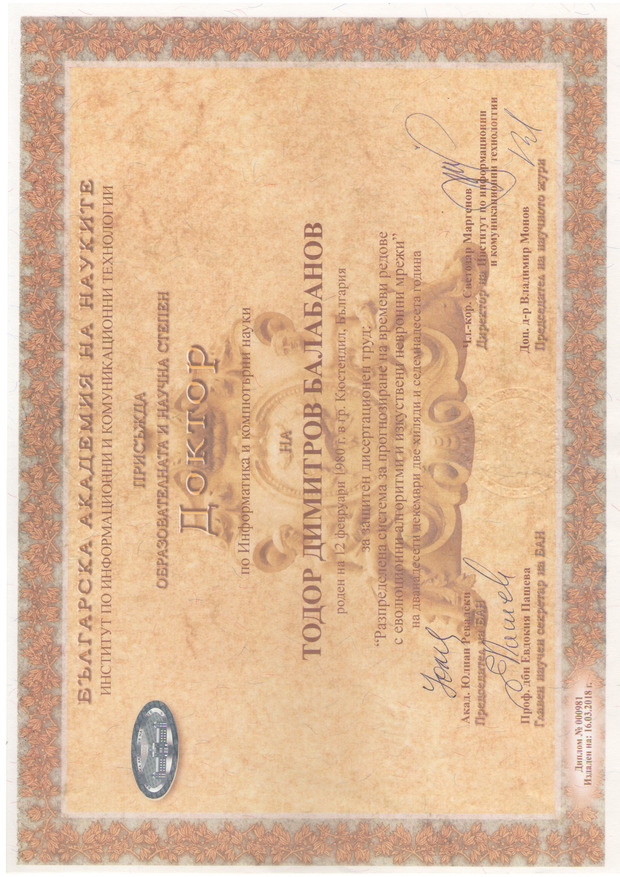
\includegraphics[width=\textwidth,height=\textheight,keepaspectratio]{DiplomaIICT2018}
%
%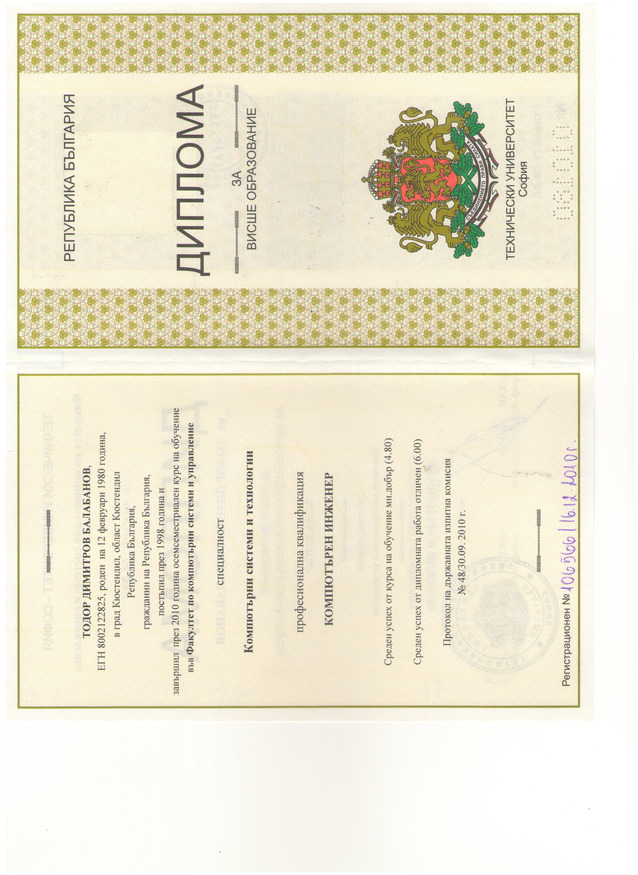
\includegraphics[width=\textwidth,height=\textheight,keepaspectratio]{DiplomaTU2010_1}
%
%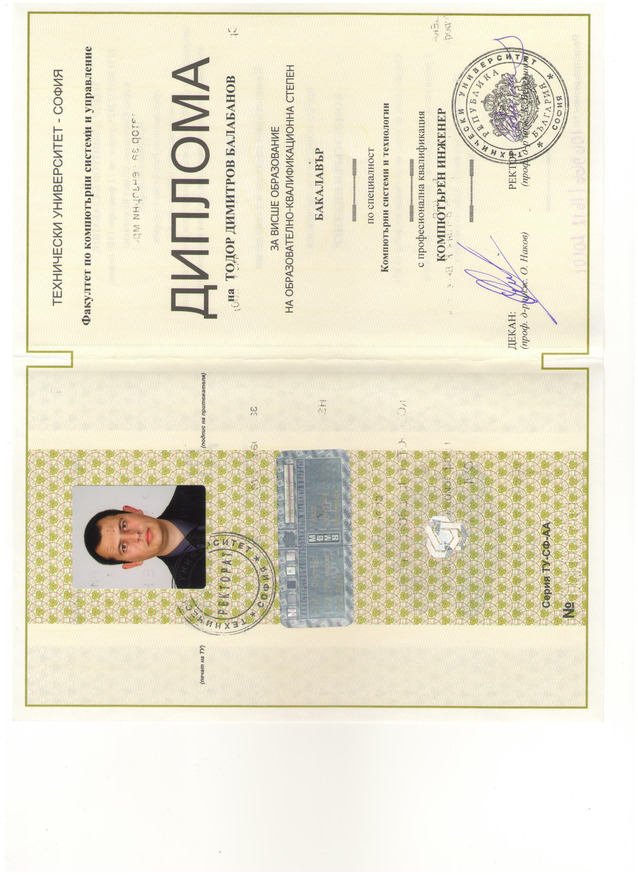
\includegraphics[width=\textwidth,height=\textheight,keepaspectratio]{DiplomaTU2010_2}
%
%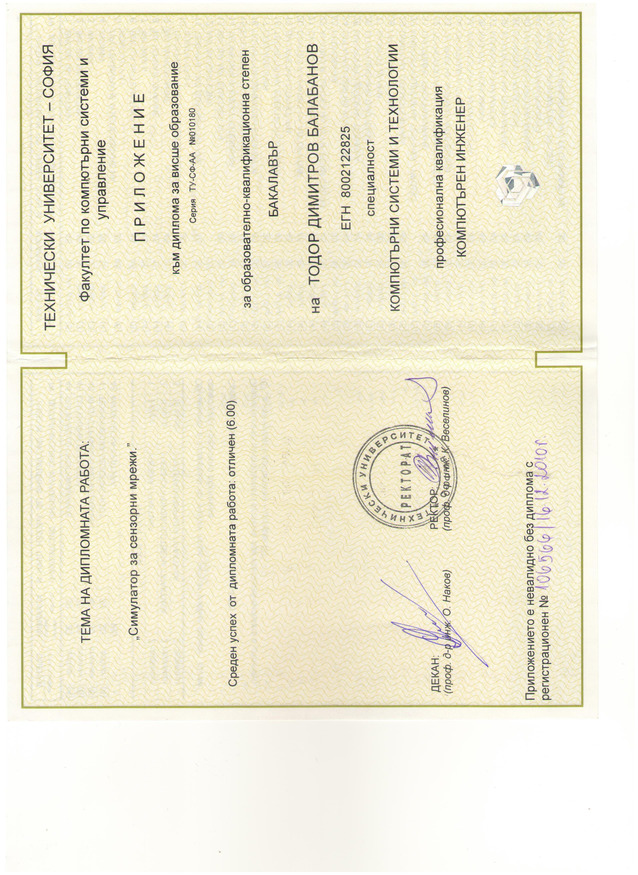
\includegraphics[width=\textwidth,height=\textheight,keepaspectratio]{DiplomaTU2010_3}
%
%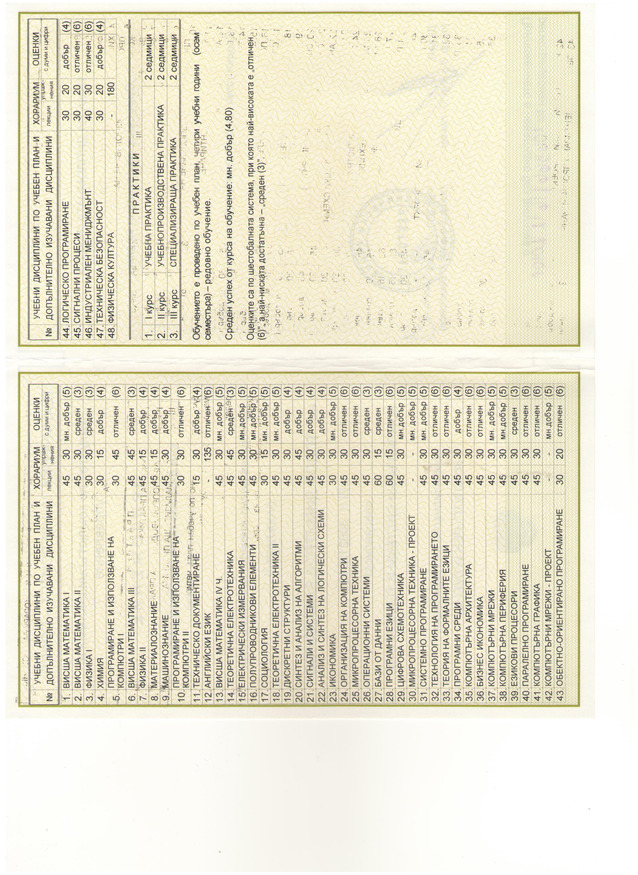
\includegraphics[width=\textwidth,height=\textheight,keepaspectratio]{DiplomaTU2010_4}
%
%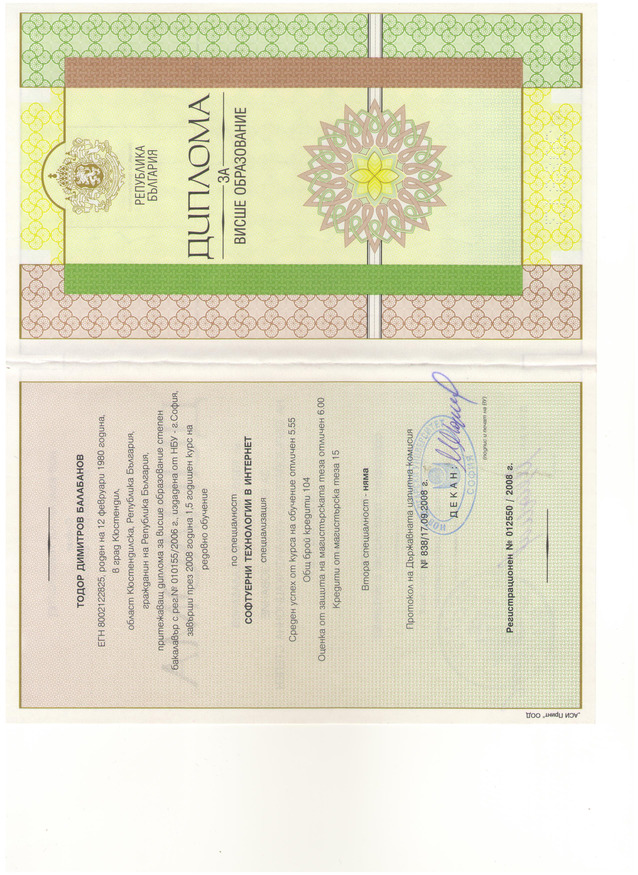
\includegraphics[width=\textwidth,height=\textheight,keepaspectratio]{DiplomaNBU2008_1}
%
%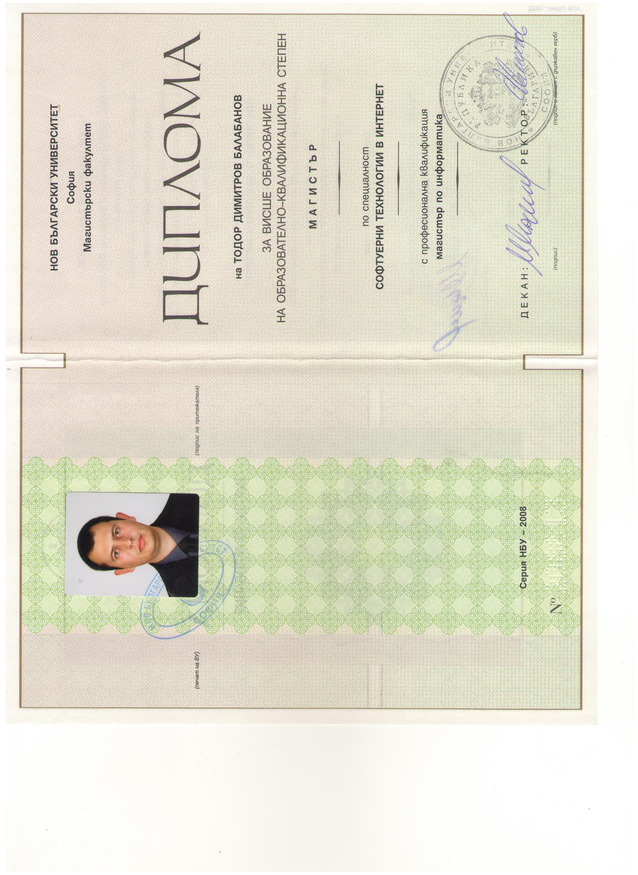
\includegraphics[width=\textwidth,height=\textheight,keepaspectratio]{DiplomaNBU2008_2}
%
%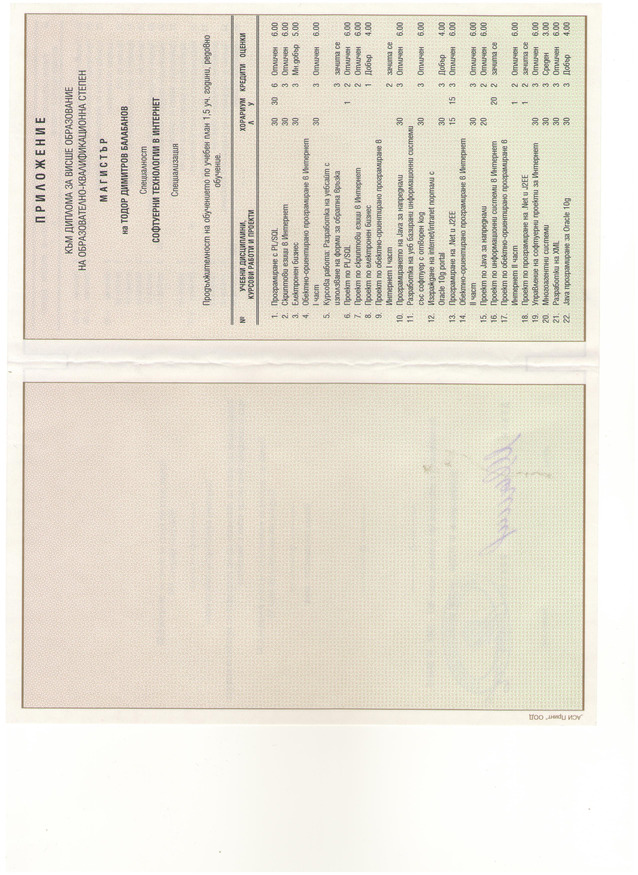
\includegraphics[width=\textwidth,height=\textheight,keepaspectratio]{DiplomaNBU2008_3}
%
%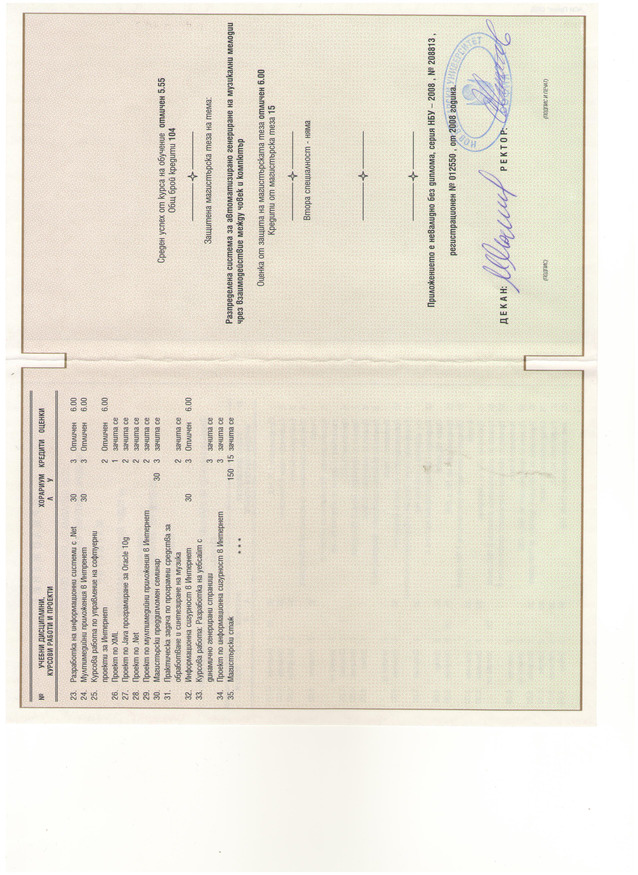
\includegraphics[width=\textwidth,height=\textheight,keepaspectratio]{DiplomaNBU2008_4}
%
%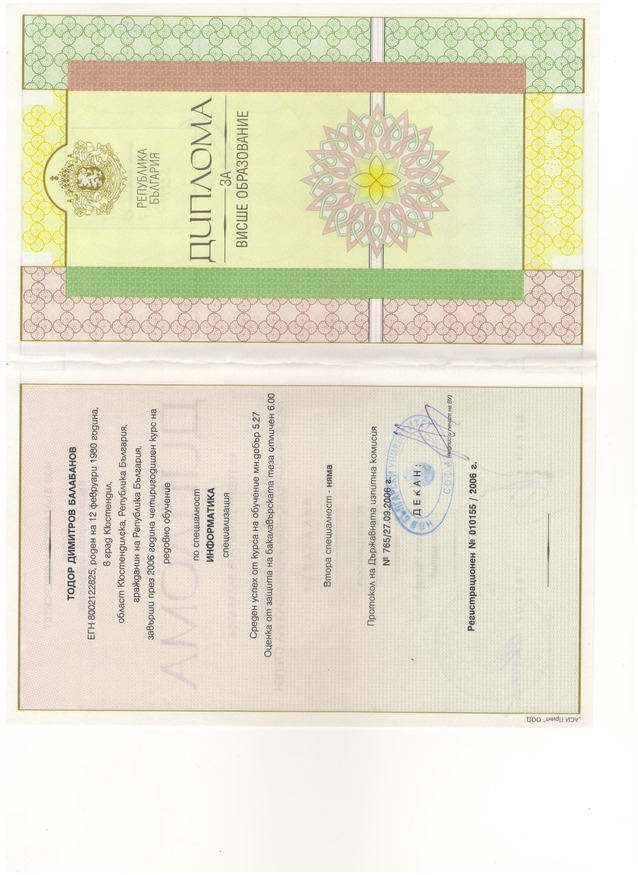
\includegraphics[width=\textwidth,height=\textheight,keepaspectratio]{DiplomaNBU2006_1}
%
%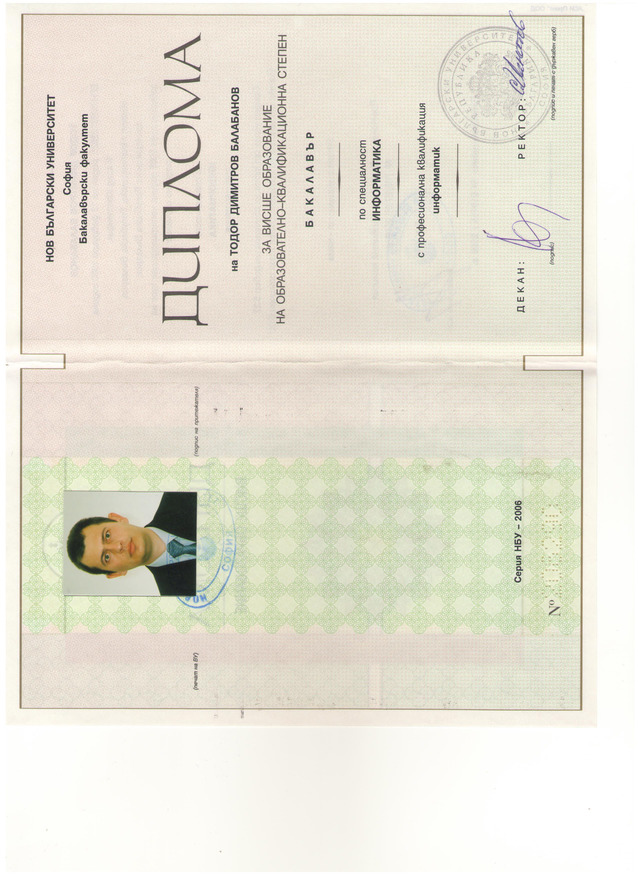
\includegraphics[width=\textwidth,height=\textheight,keepaspectratio]{DiplomaNBU2006_2}
%
%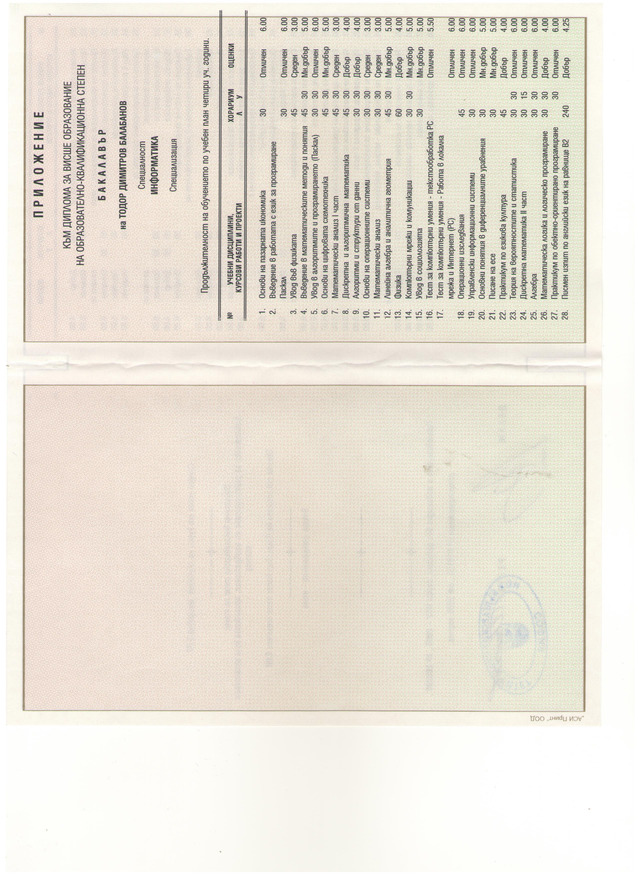
\includegraphics[width=\textwidth,height=\textheight,keepaspectratio]{DiplomaNBU2006_3}
%
%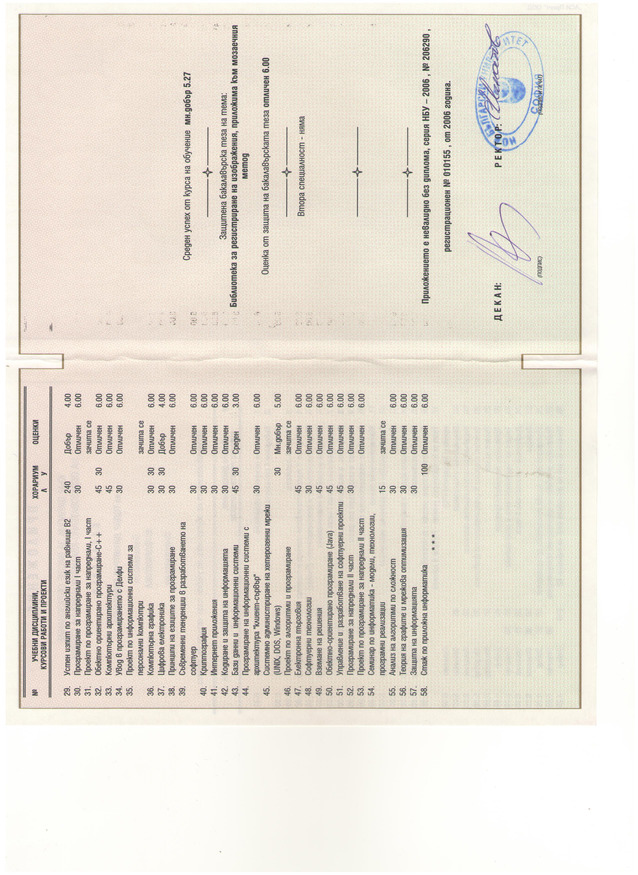
\includegraphics[width=\textwidth,height=\textheight,keepaspectratio]{DiplomaNBU2006_4}
%
%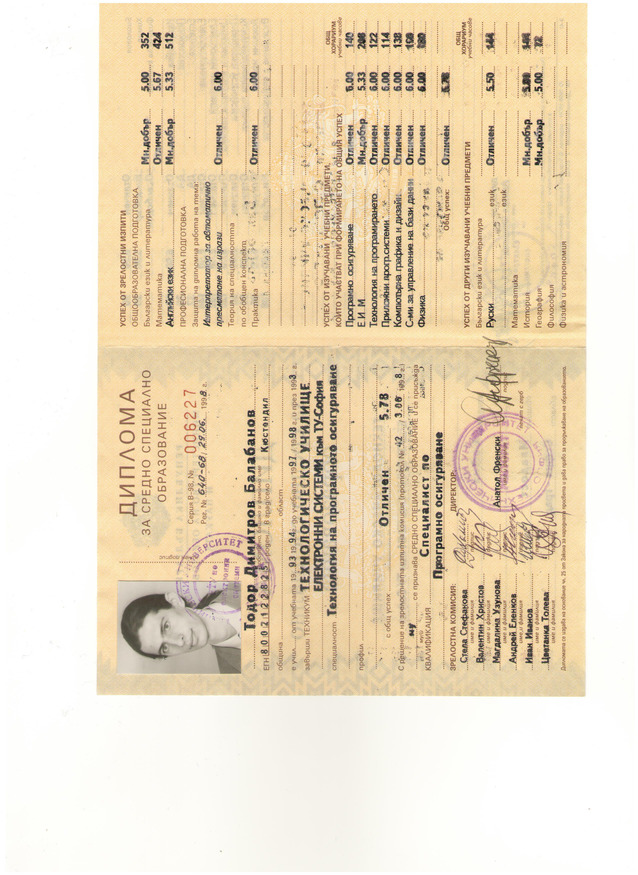
\includegraphics[width=\textwidth,height=\textheight,keepaspectratio]{DiplomaTUES1998_1}
%
%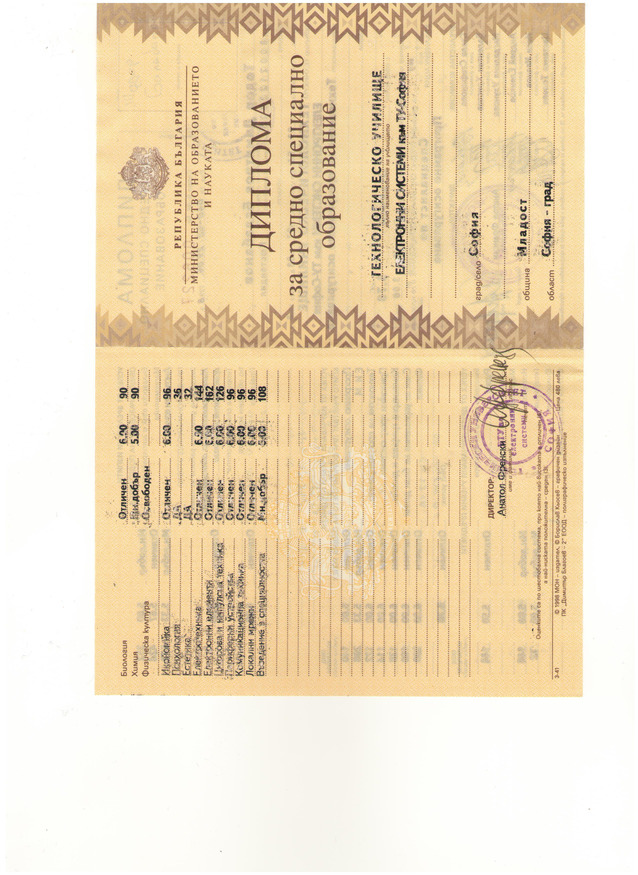
\includegraphics[width=\textwidth,height=\textheight,keepaspectratio]{DiplomaTUES1998_2}
%
%%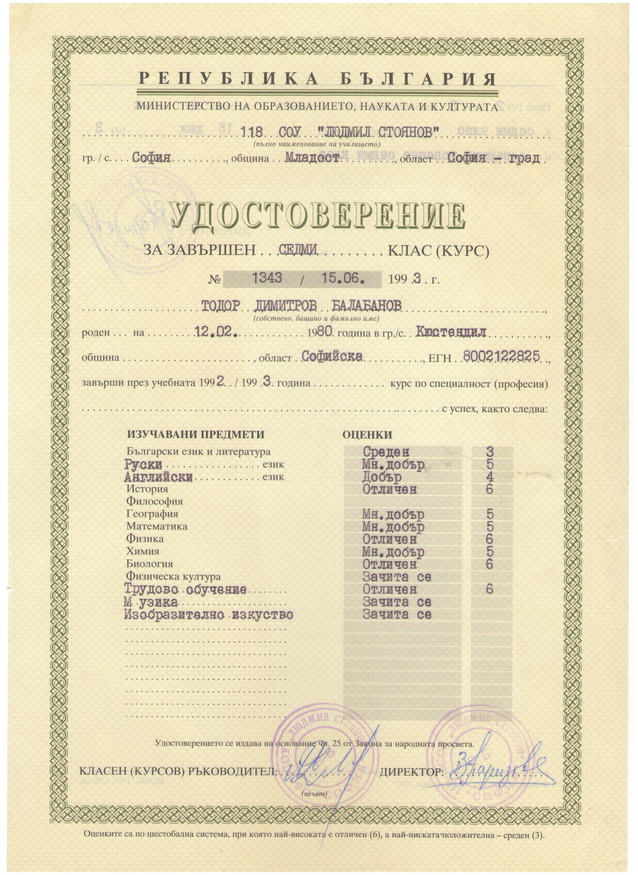
\includegraphics[width=\textwidth,height=\textheight,keepaspectratio]{118SOU1993_1}
%
%%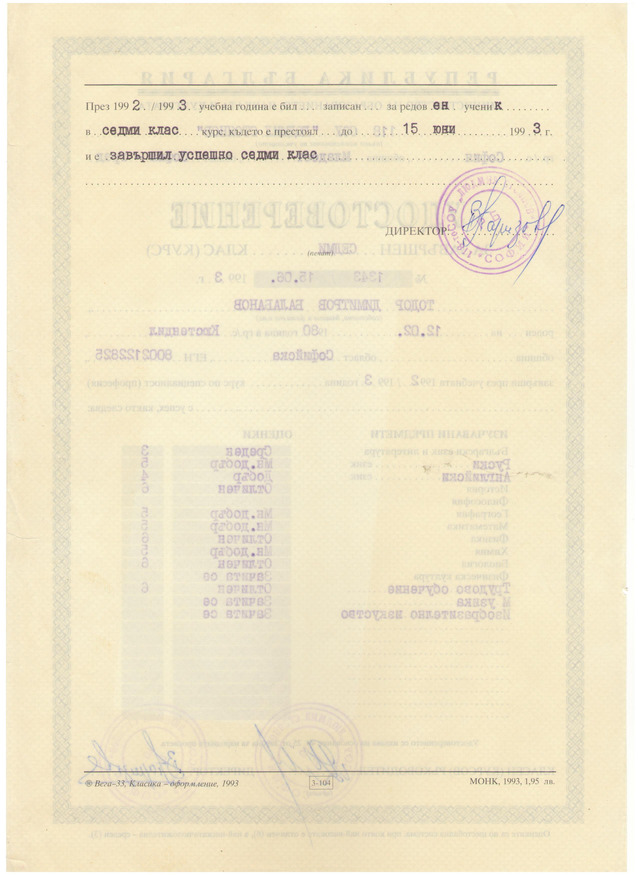
\includegraphics[width=\textwidth,height=\textheight,keepaspectratio]{118SOU1993_2}
%
%%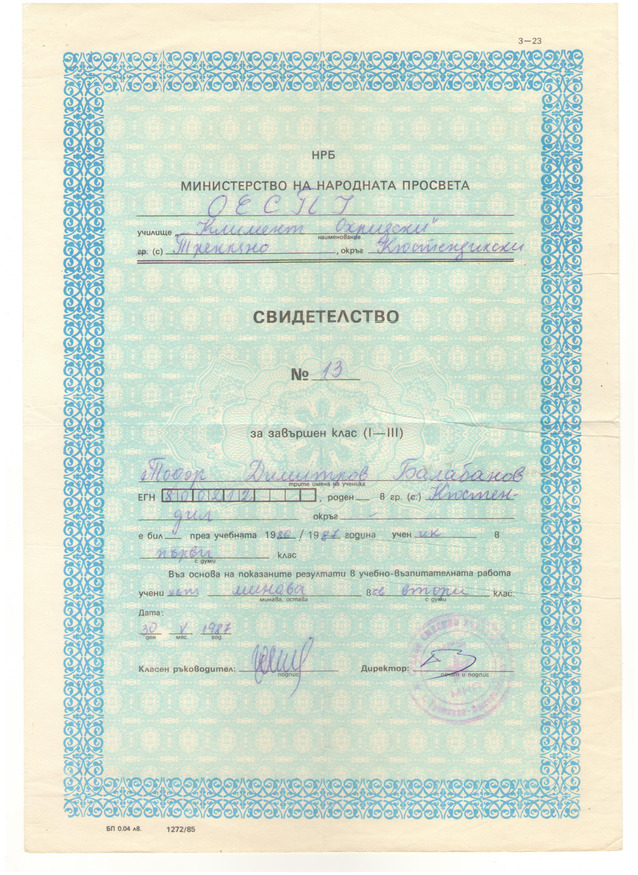
\includegraphics[width=\textwidth,height=\textheight,keepaspectratio]{OESPU1987}
%
%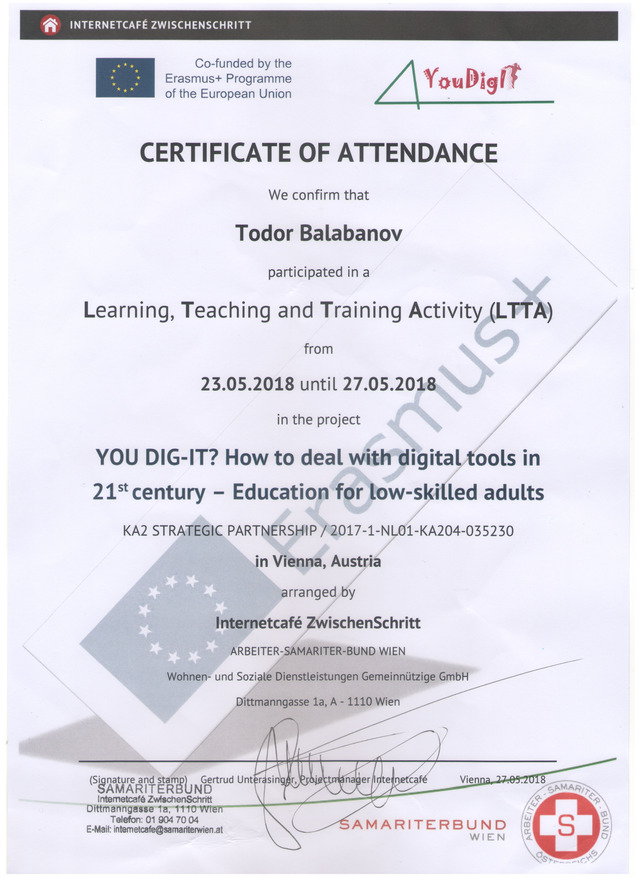
\includegraphics[width=\textwidth,height=\textheight,keepaspectratio]{YouDigIT2018}
%
%
\includegraphics[width=\textwidth,height=\textheight,keepaspectratio]{ESGI1322017}
%
%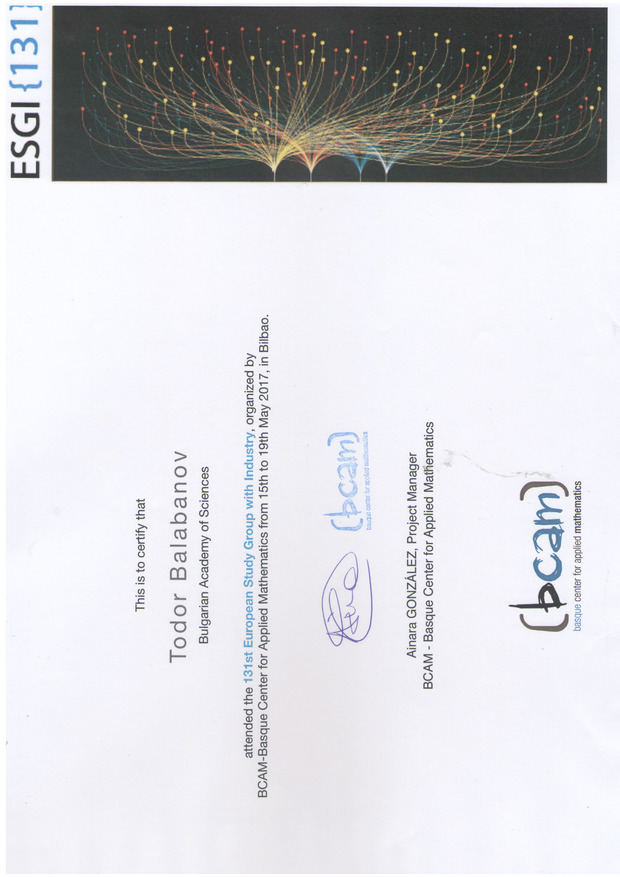
\includegraphics[width=\textwidth,height=\textheight,keepaspectratio]{131ESGI2017}
%
%
\includegraphics[width=\textwidth,height=\textheight,keepaspectratio]{KNSB2017_1}
%
%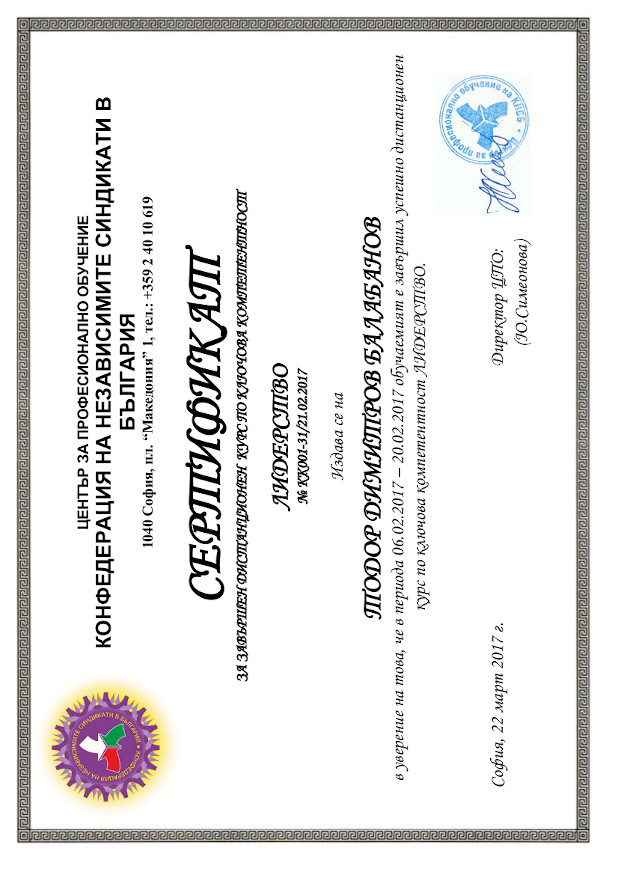
\includegraphics[width=\textwidth,height=\textheight,keepaspectratio]{KNSB2017_2}
%
%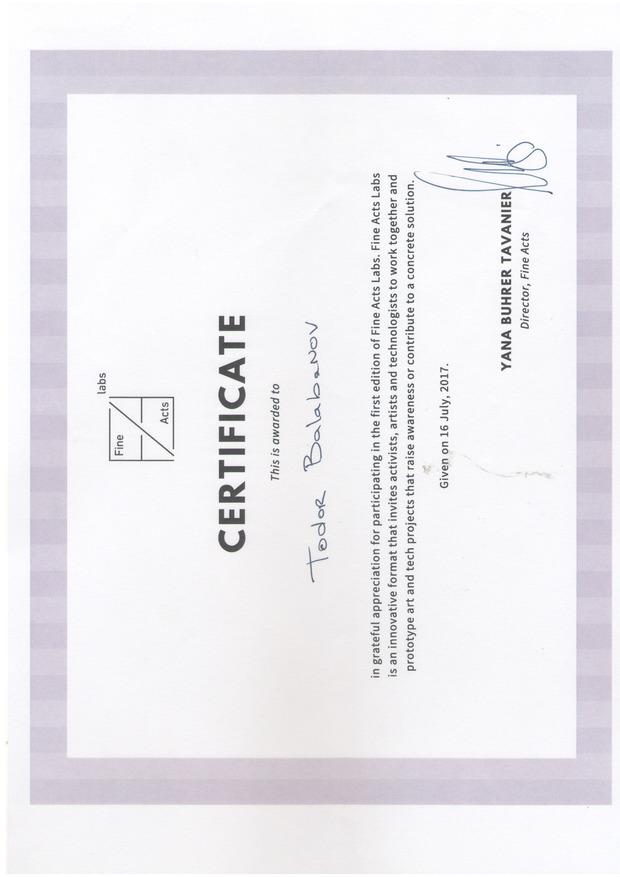
\includegraphics[width=\textwidth,height=\textheight,keepaspectratio]{FineActsLabs2017}
%
%
\includegraphics[width=\textwidth,height=\textheight,keepaspectratio]{InfoTech2016}
%
%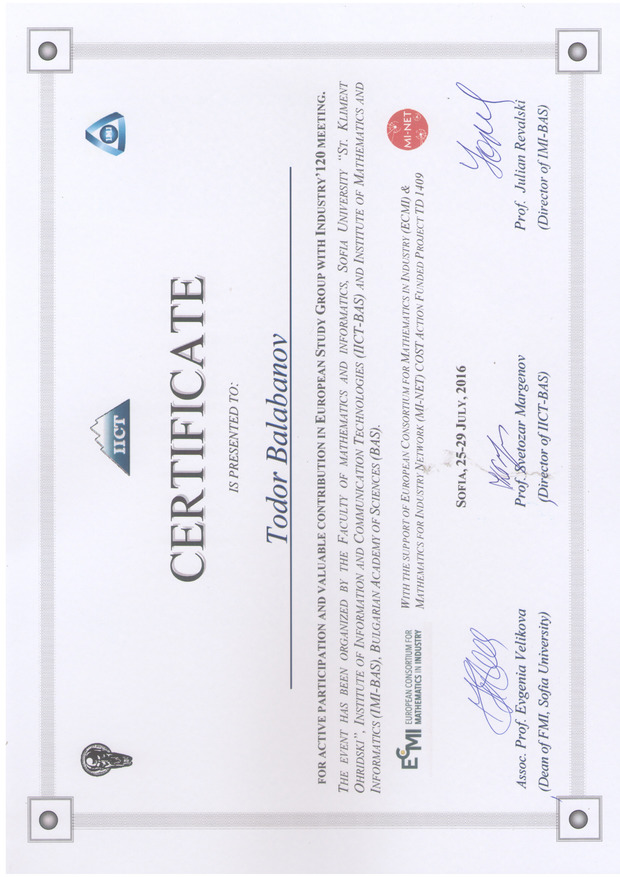
\includegraphics[width=\textwidth,height=\textheight,keepaspectratio]{ESGI1202016}
%
%
\includegraphics[width=\textwidth,height=\textheight,keepaspectratio]{MA2016}
%
%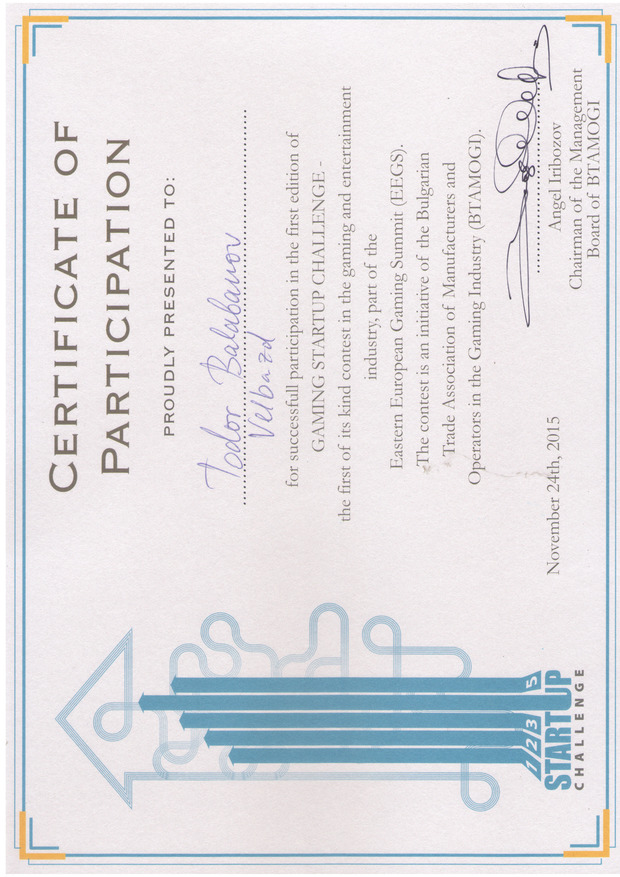
\includegraphics[width=\textwidth,height=\textheight,keepaspectratio]{EEGS2015}
%
%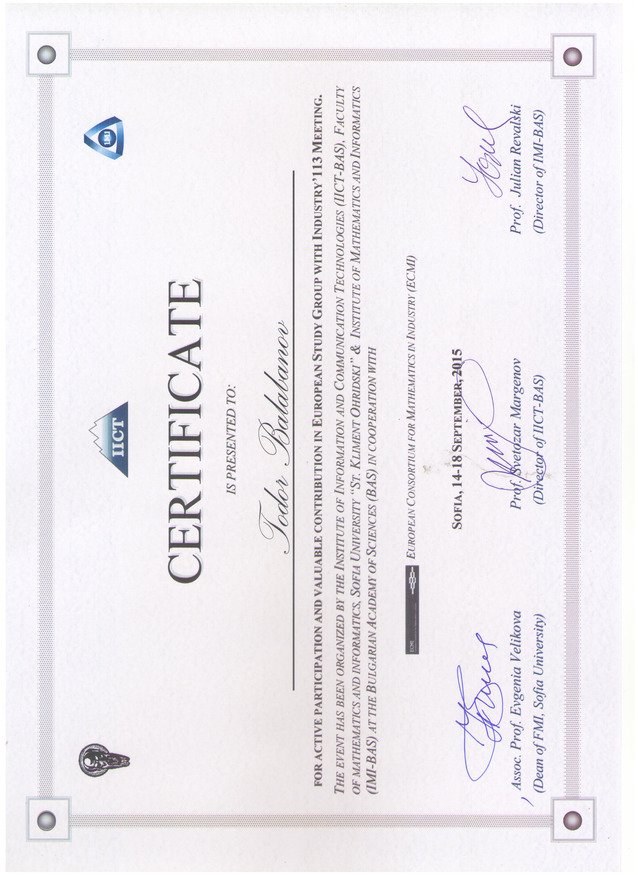
\includegraphics[width=\textwidth,height=\textheight,keepaspectratio]{ESGI1132015}
%
%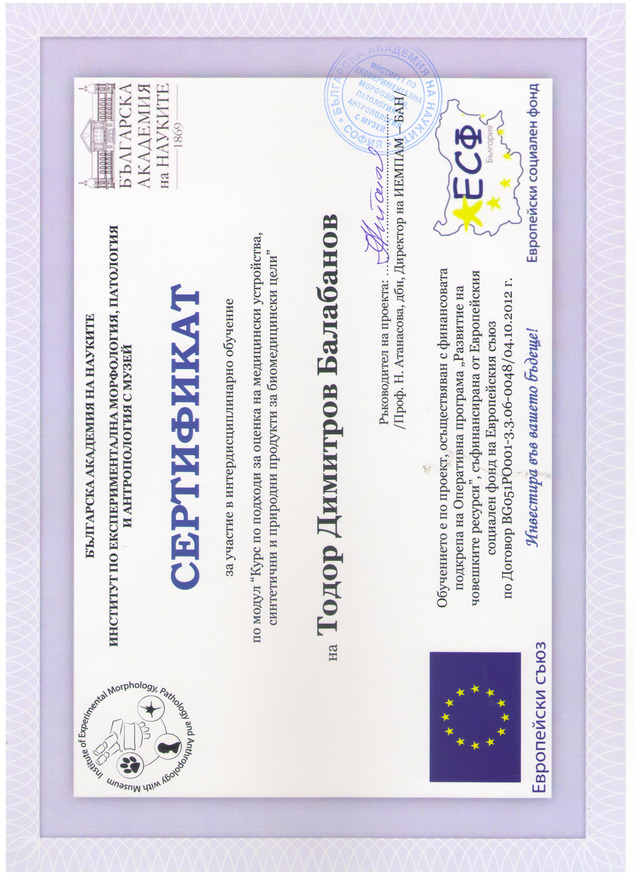
\includegraphics[width=\textwidth,height=\textheight,keepaspectratio]{IEMPAM2014_1}
%
%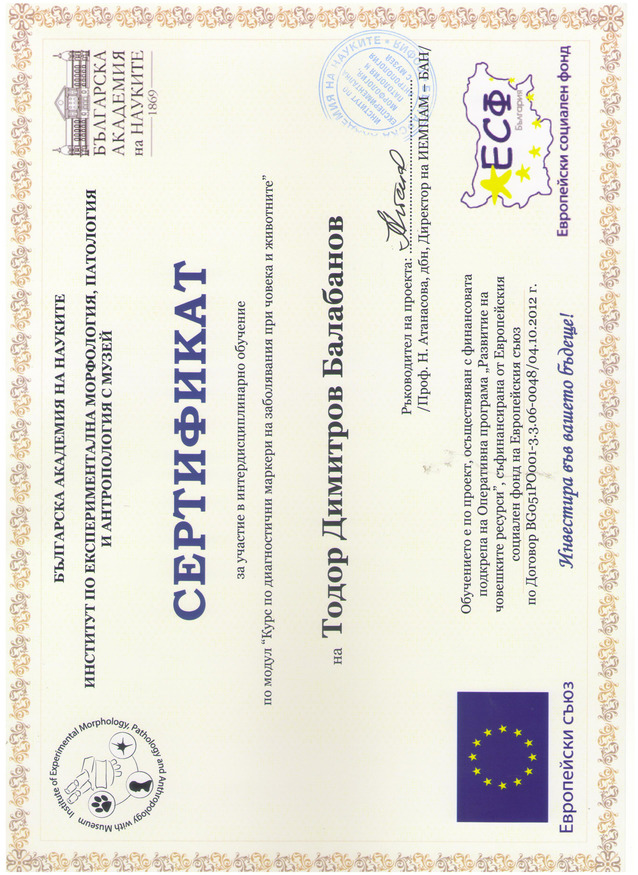
\includegraphics[width=\textwidth,height=\textheight,keepaspectratio]{IEMPAM2014_2}
%
%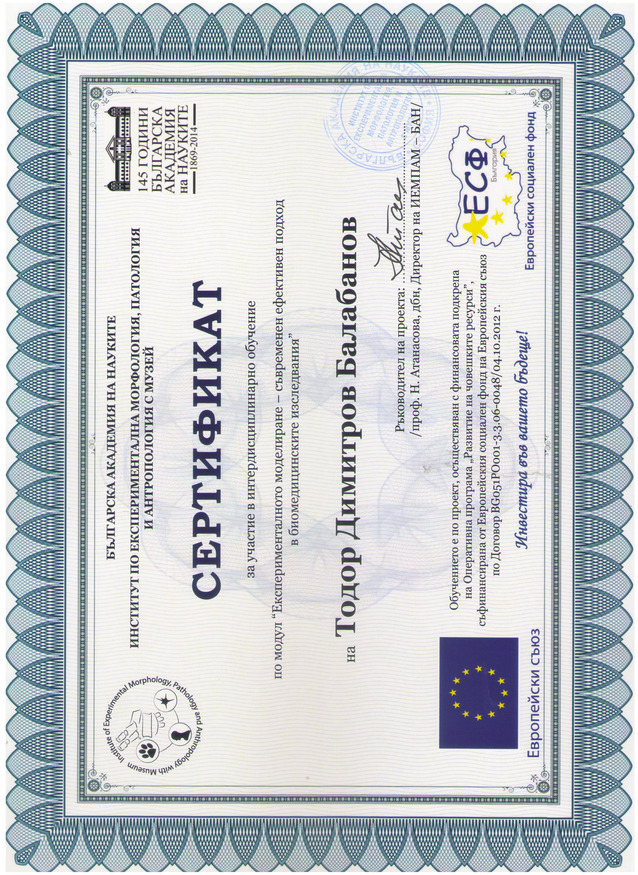
\includegraphics[width=\textwidth,height=\textheight,keepaspectratio]{IEMPAM2014_3}
%
%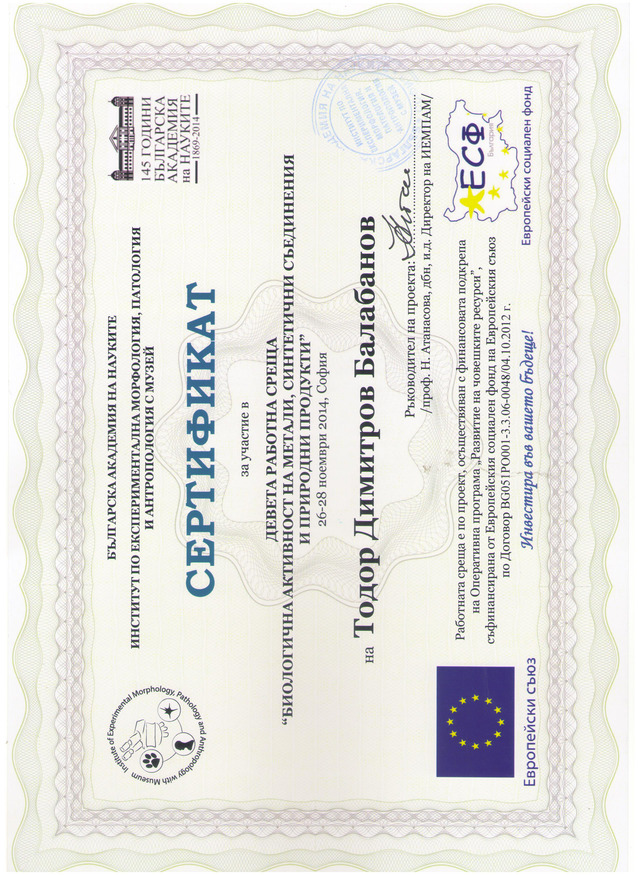
\includegraphics[width=\textwidth,height=\textheight,keepaspectratio]{IEMPAM2014_4}
%
%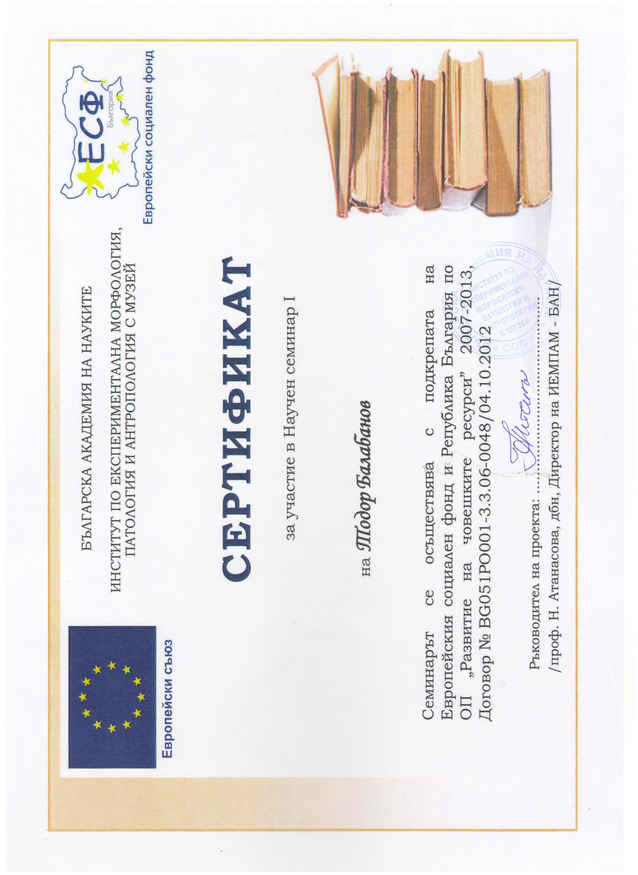
\includegraphics[width=\textwidth,height=\textheight,keepaspectratio]{IEMPAM2013_1}
%
%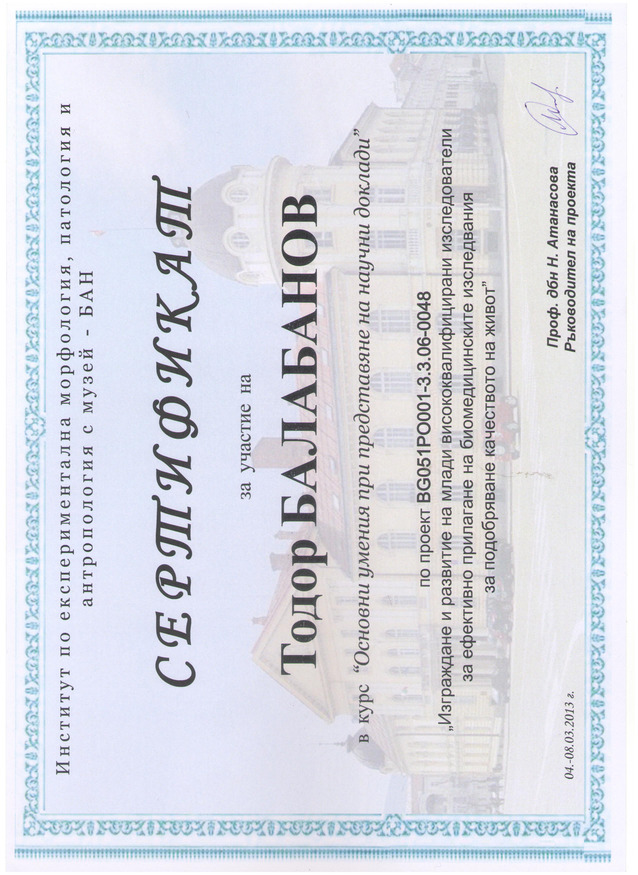
\includegraphics[width=\textwidth,height=\textheight,keepaspectratio]{IEMPAM2013_2}
%
%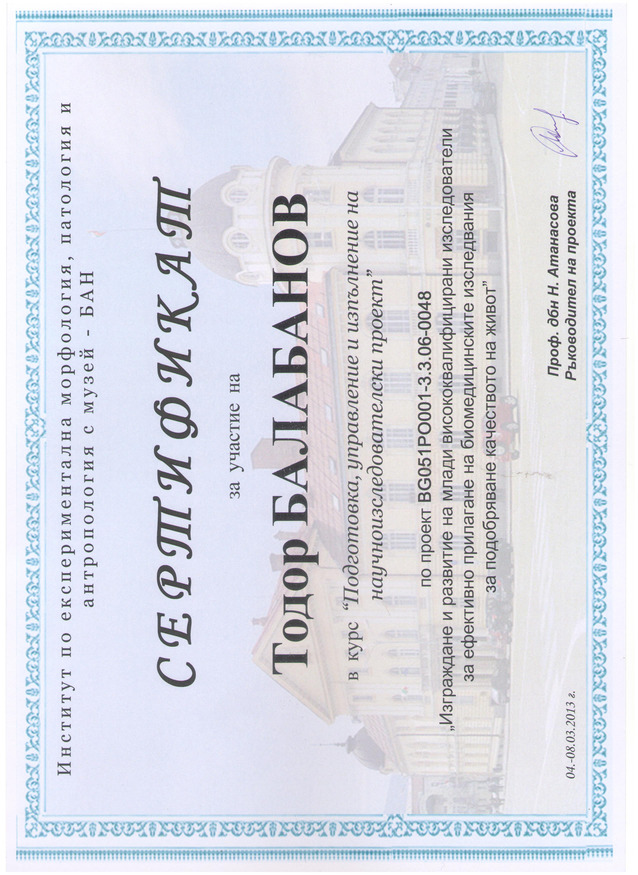
\includegraphics[width=\textwidth,height=\textheight,keepaspectratio]{IEMPAM2013_3}
%
%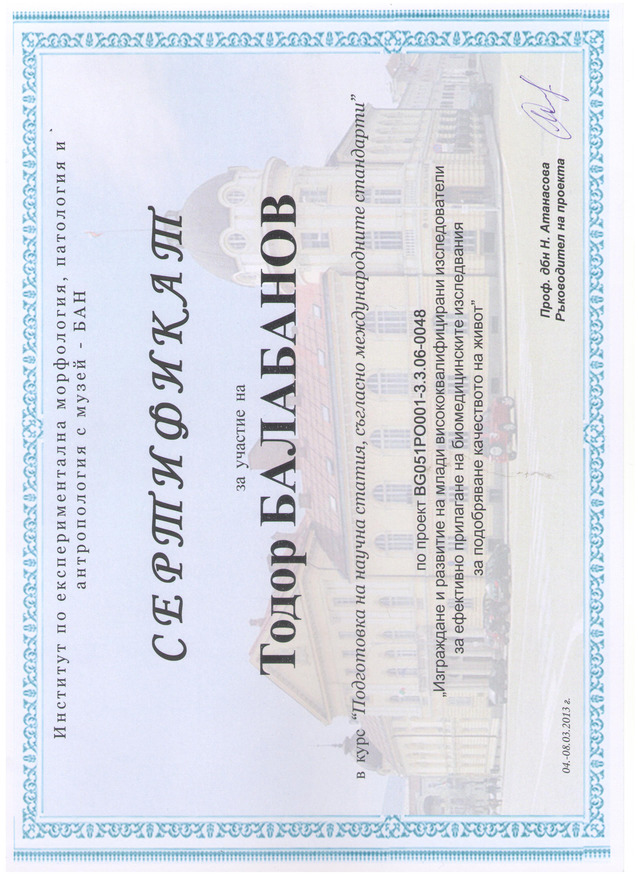
\includegraphics[width=\textwidth,height=\textheight,keepaspectratio]{IEMPAM2013_4}
%
%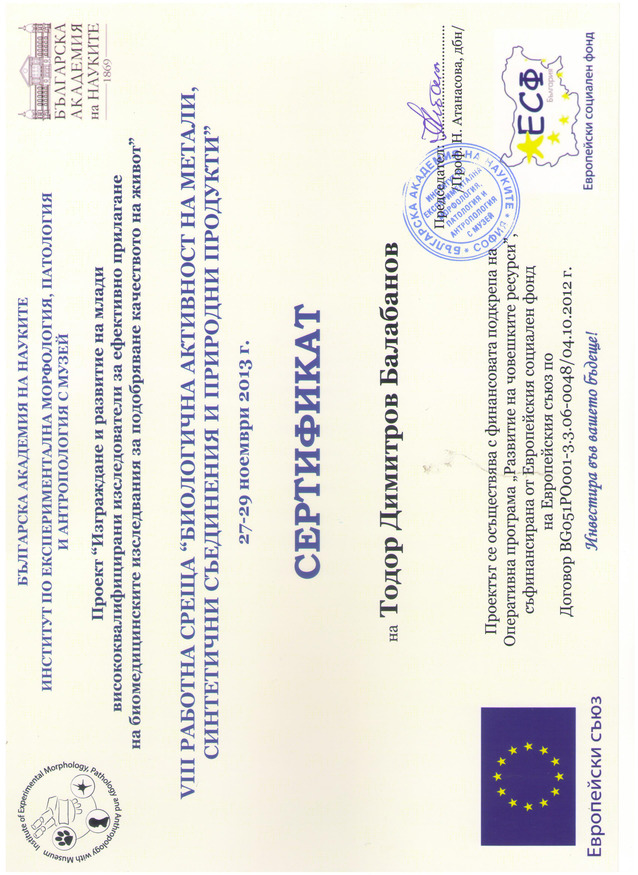
\includegraphics[width=\textwidth,height=\textheight,keepaspectratio]{IEMPAM2013_5}
%
%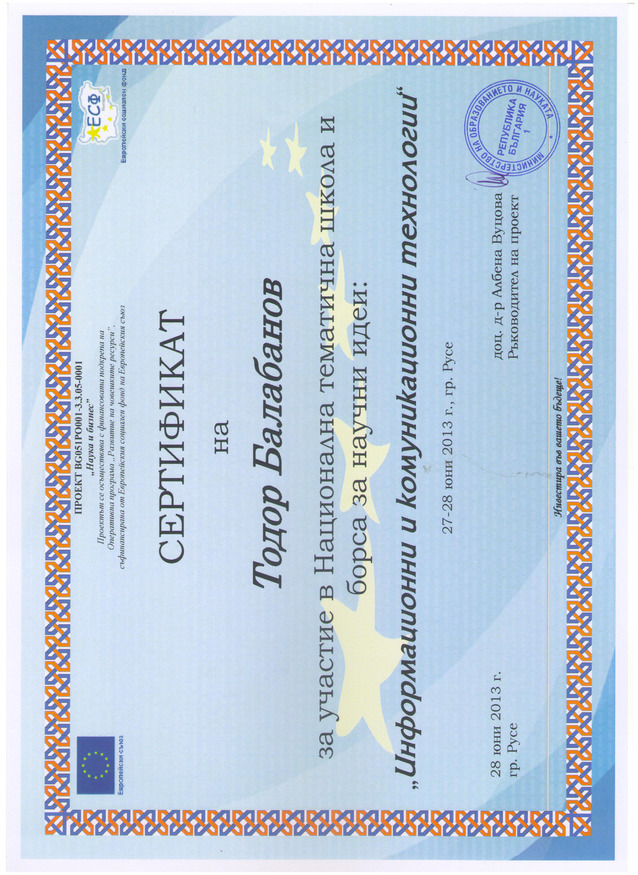
\includegraphics[width=\textwidth,height=\textheight,keepaspectratio]{Rouse2013}
%
%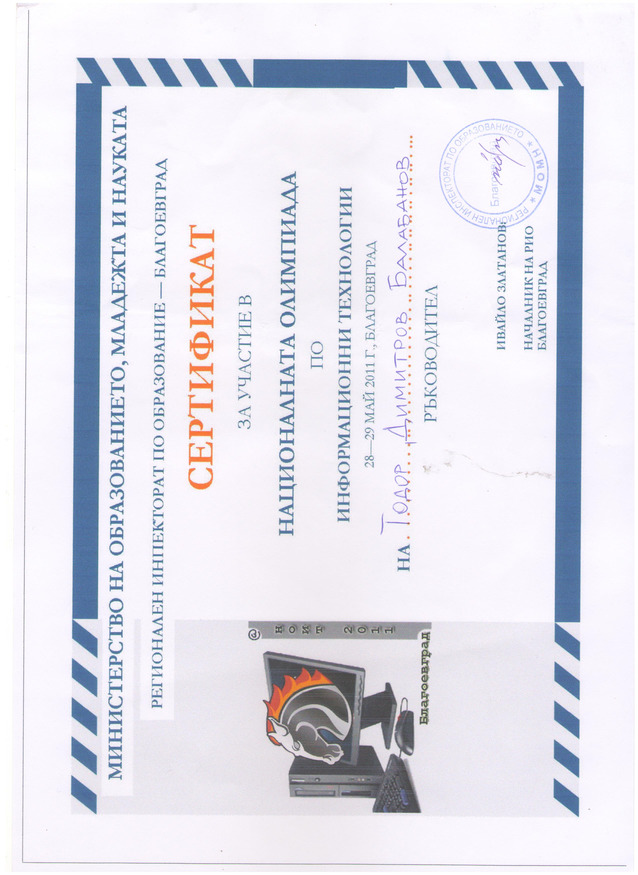
\includegraphics[width=\textwidth,height=\textheight,keepaspectratio]{ElSys2011}
%
%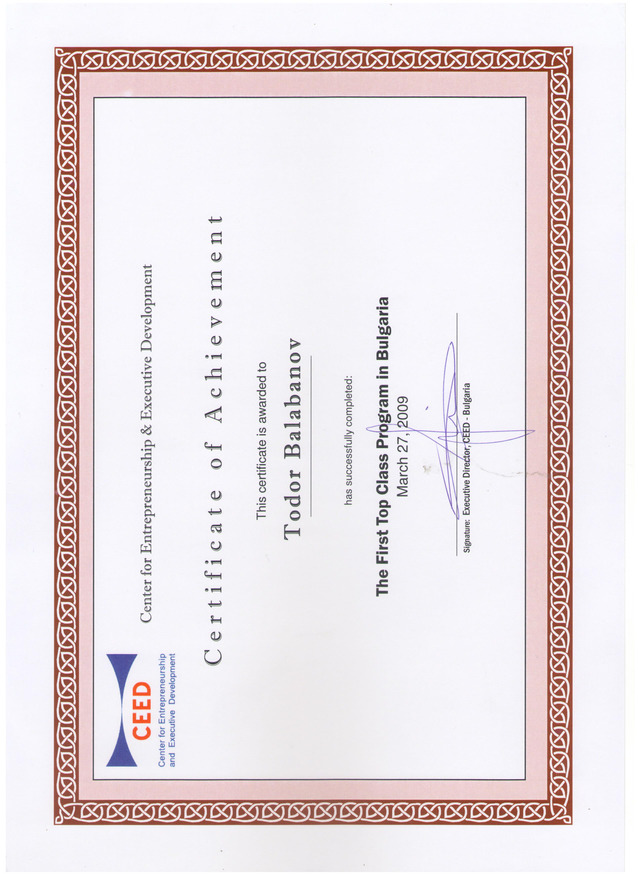
\includegraphics[width=\textwidth,height=\textheight,keepaspectratio]{CEED2009}
%
%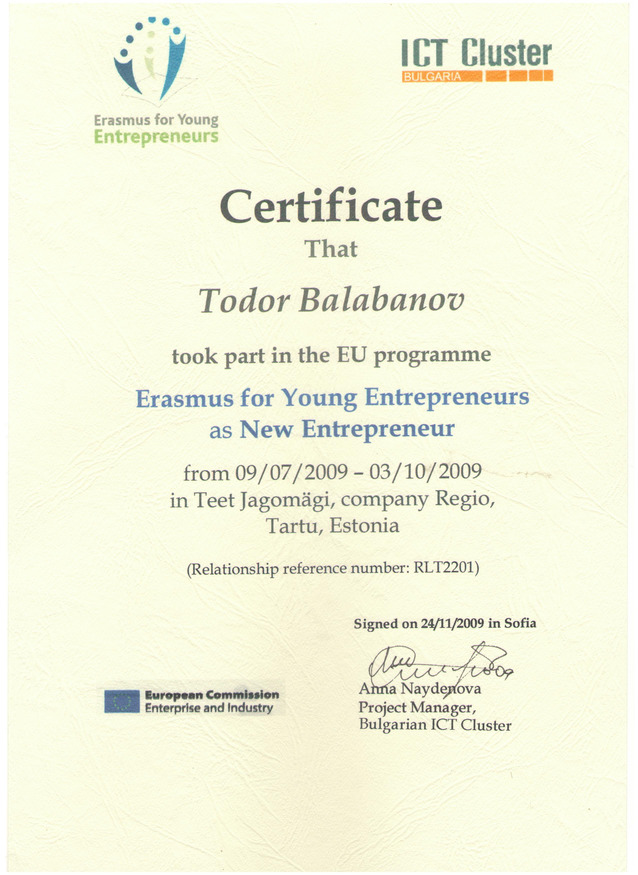
\includegraphics[width=\textwidth,height=\textheight,keepaspectratio]{EYE2009}
%
%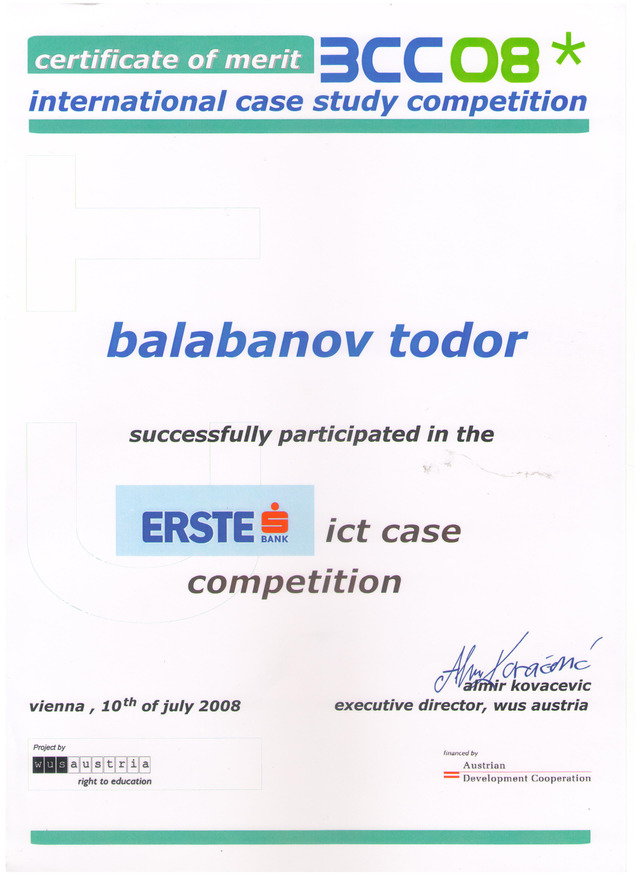
\includegraphics[width=\textwidth,height=\textheight,keepaspectratio]{BCC2008}
%
%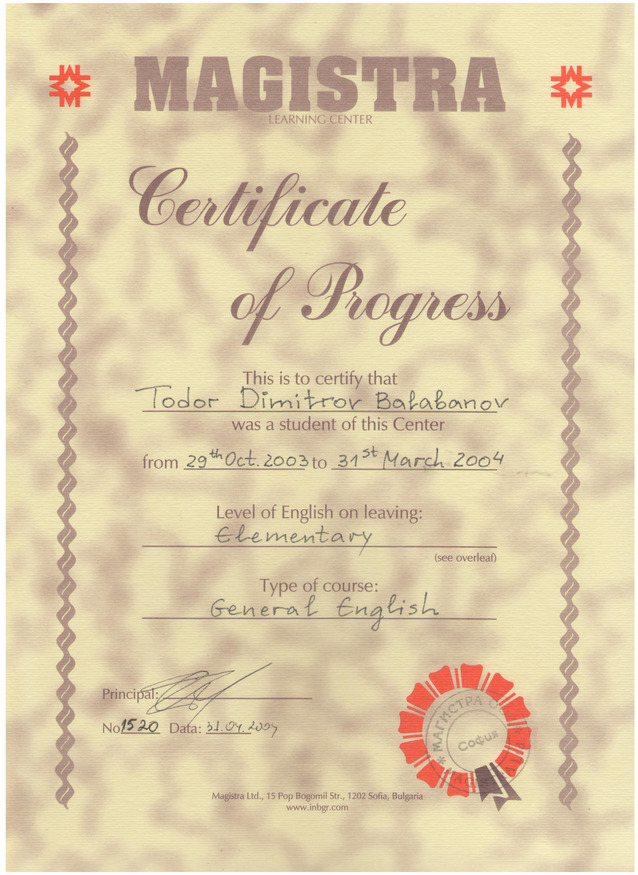
\includegraphics[width=\textwidth,height=\textheight,keepaspectratio]{Magistra2004}
%
%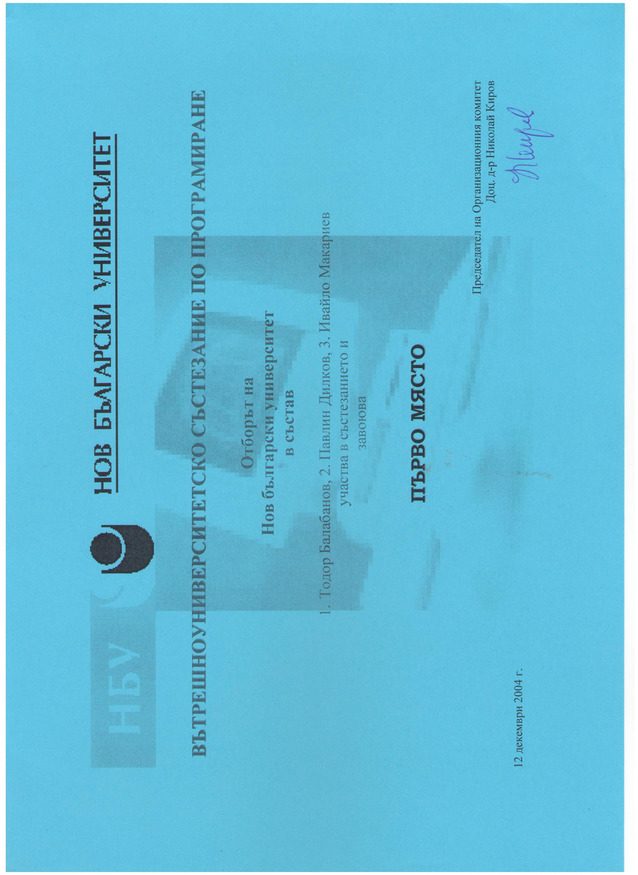
\includegraphics[width=\textwidth,height=\textheight,keepaspectratio]{NBU2004}
%
%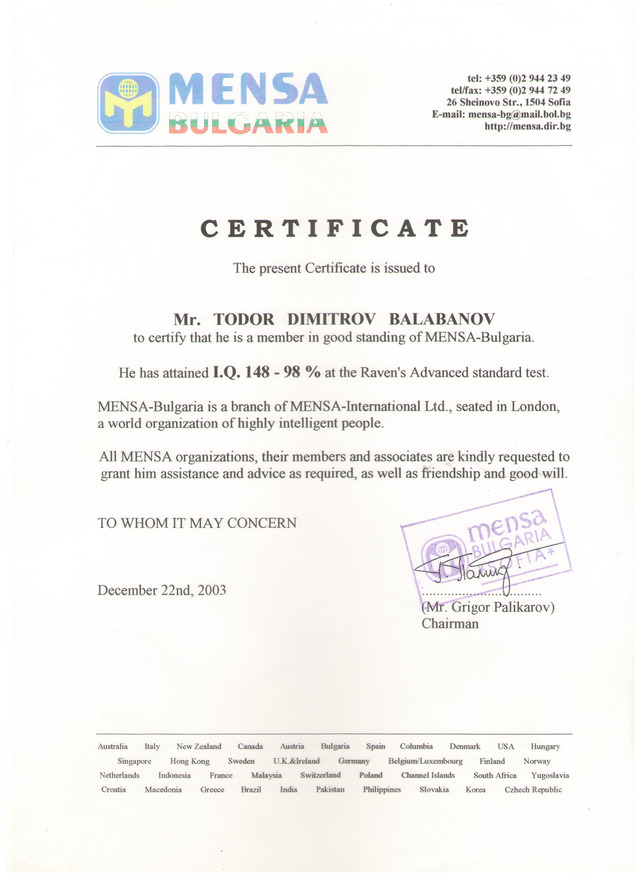
\includegraphics[width=\textwidth,height=\textheight,keepaspectratio]{Mensa2003}
%
%%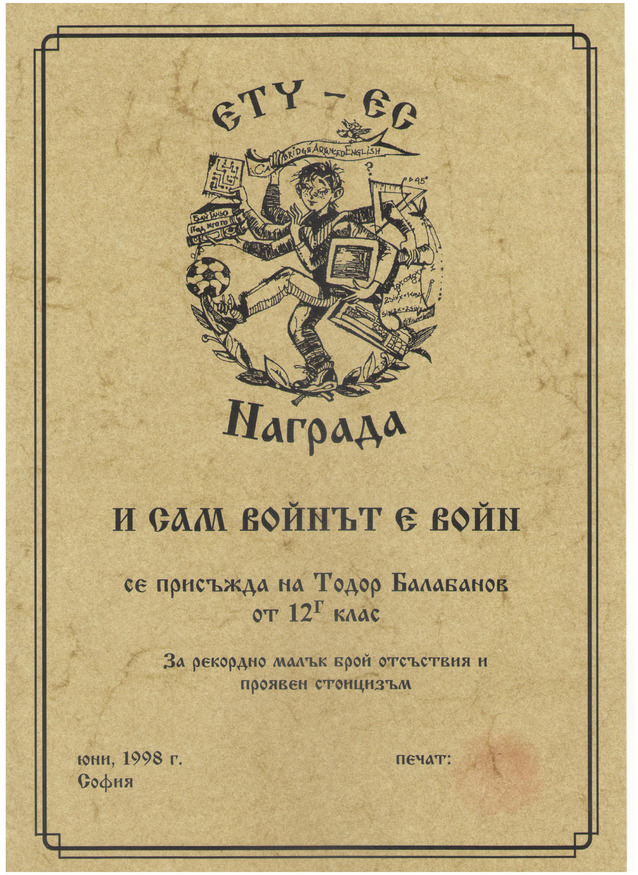
\includegraphics[width=\textwidth,height=\textheight,keepaspectratio]{ElSys1998}
%
%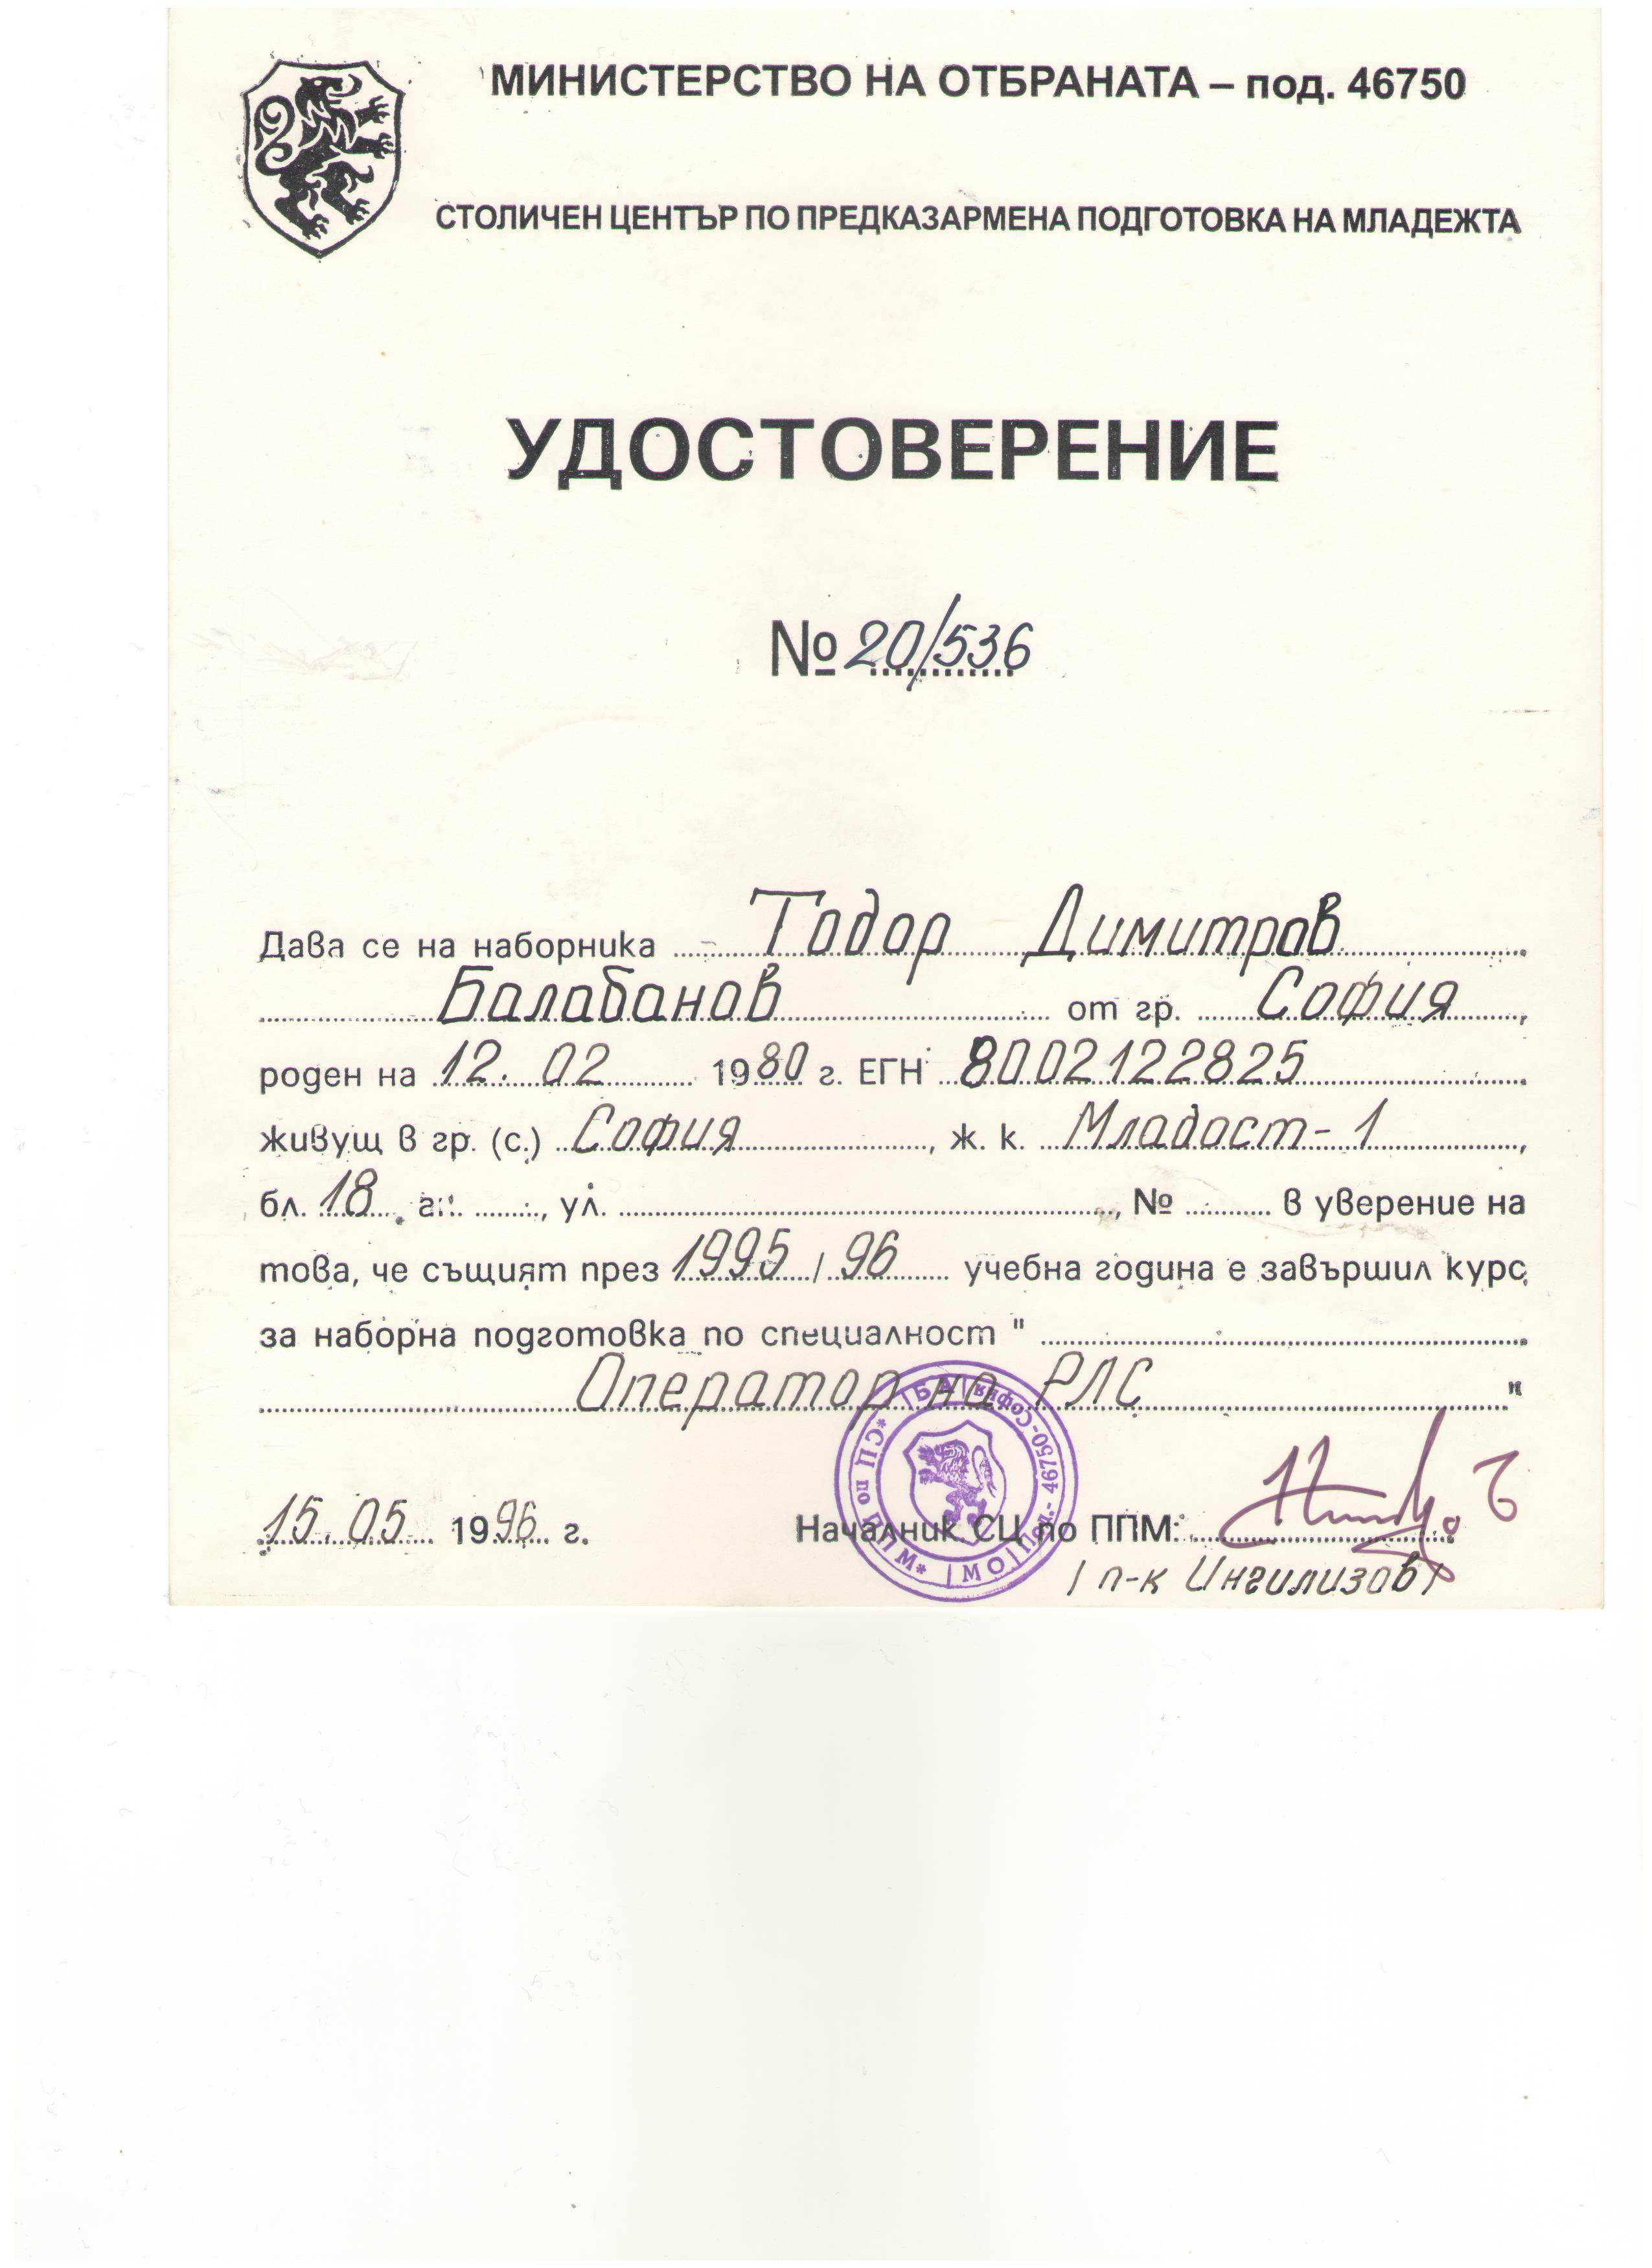
\includegraphics[width=\textwidth,height=\textheight,keepaspectratio]{MO1996}

\end{document}
